\section{Numerical Simulations}


%%%%%%%%%%%%%%%%%%%%%%%%%%%%%%%%%%%%%%%%%%%%%%%%%%%%%%%%%%%%%%%%
%%%%%%%%%%%%%%%%%%%%%%%%%%%%%%%%%%%%%%%%%%%%%%%%%%%%%%%%%%%%%%%%
%%%%%%%%%%%%%%%%%%%%%%%%%%%%%%%%%%%%%%%%%%%%%%%%%%%%%%%%%%%%%%%%
\subsection{Comparison of Proximal Schemes}

This Section compares the following algorithms introduced in Section~\ref{sec-proximal}:\vspace{-0.1cm}
\begin{itemize} 
	\item Douglas-Rachford (DR in the following) as exposed in Section~\ref{DR-algo}, parameterized with $\al$ and $\ga$ ;
	\item ADDM on the dual (ADDM in the following) introduced in~\cite{Benamou2000}, (which is DR with $\al=1$) parameterized with $\ga$ ; 
	\item Primal-dual (PD in the following) as exposed in Section~\ref{PD-algo}, parameterized with $\si$ and $\tau$.\vspace{-0.1cm}
\end{itemize}

The comparison is done on a simple example with two 2-D isotropic Gaussian distributions $(f^0,f^1)$ with the same variance. In the continuous case, the solution is known to be a translation between the mean of the Gaussians. The spatial domain is here of dimension $d=2$ and it is discretized on a grid with $N=M=31$ points for both each dimension. The temporal  discretization has also been fixed to $P=31$. We first compute an (almost) exact reference solution $(m^\star,f^\star)$ of the discrete problem with $10^6$ iterations of the DR. The obtained transported mass $f^\star(\cdot,t)$ is illustrated in Figure \ref{fig:data_bump}.

\begin{figure}[!ht]
\begin{center}
\begin{tabular}{ccccc}
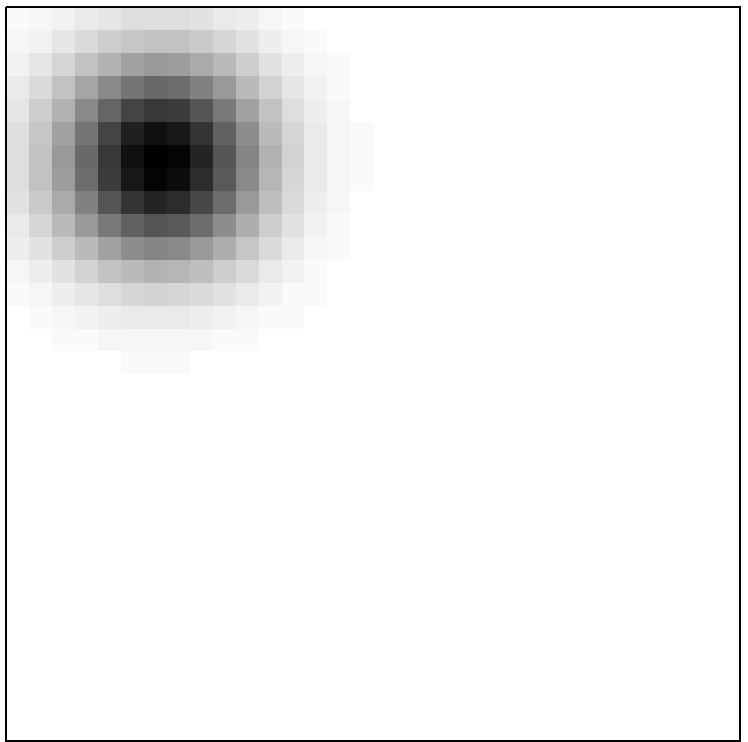
\includegraphics[width=2.5cm]{images/bump_betaold/bump_beta1_01}&
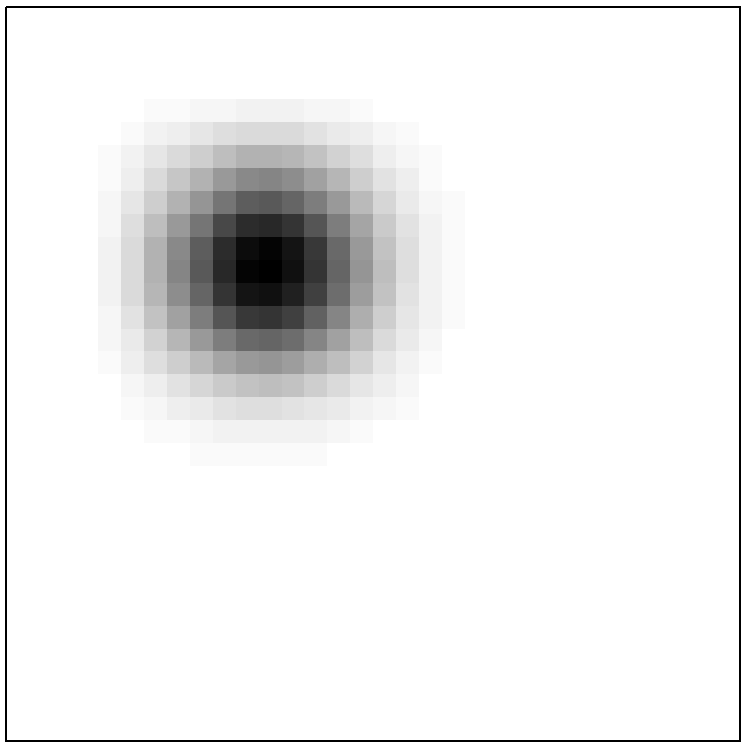
\includegraphics[width=2.5cm]{images/bump_betaold/bump_beta1_09}&
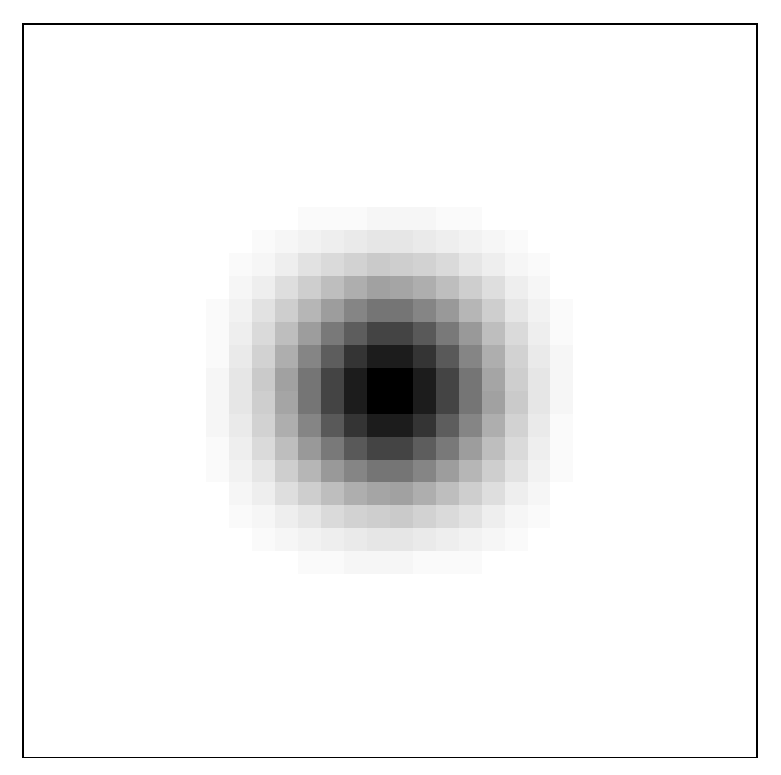
\includegraphics[width=2.5cm]{images/bump_betaold/bump_beta1_17}&
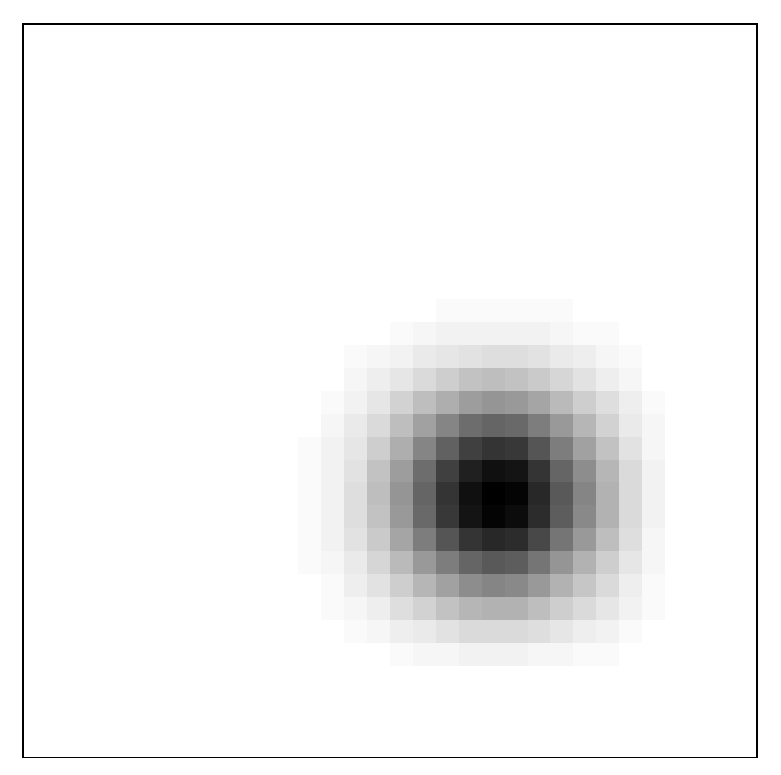
\includegraphics[width=2.5cm]{images/bump_betaold/bump_beta1_25}&
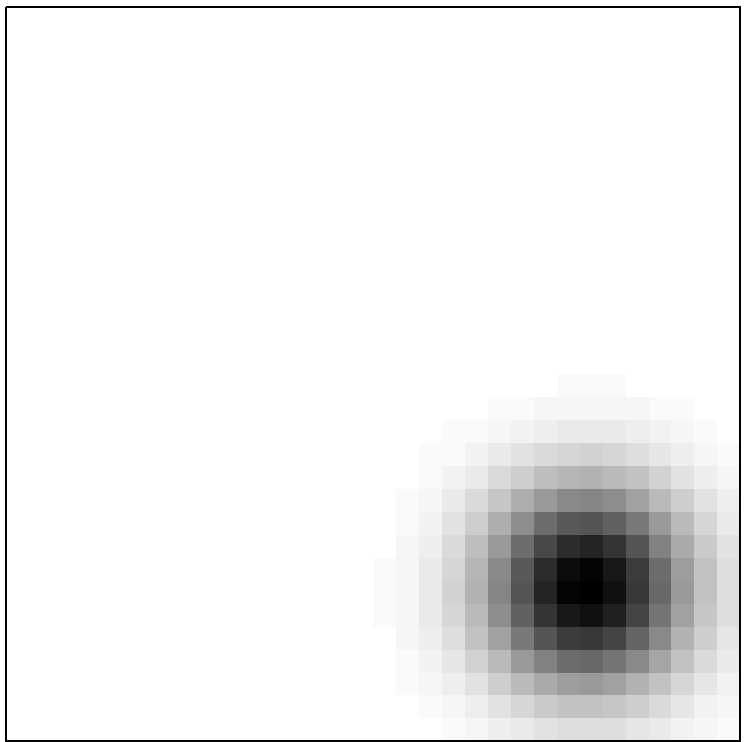
\includegraphics[width=2.5cm]{images/bump_betaold/bump_beta1_33}\\
$t=0$&$t=1/4$&$t=1/2$&$t=3/4$&$t=1$ % \vspace{-0.1cm}
\end{tabular}
\caption{\label{fig:data_bump} 
Display of $f^\star(\cdot,t)$ for several value of $t$ (note that for $t=0$ and $t=1$, this corresponds to $f^0$ and $f^1$). The grayscale values are linearly interpolating from black to white between 0 and the maximum value of $f^\star$. 
% \vspace{-0.2cm}% 10^{-8} 0.017
}
\end{center}
\end{figure}

For each algorithm, we perform an exhaustive search of the best possible set of parameters. These optimal parameters are those minimizing $\norm{(m^\star,f^\star) - (\iter{m},\iter{f})}$, the $\ell^2$ distance between $f^\star$ and the output of the algorithm after $\ell=100$ iterations. The obtained  parameters for this data set are:  $\ga=1/350$ for ADMM on the dual, $(\ga=1/240,\al=1.983)$ for DR and $\si=85$ for PD. For PD, we found that simply setting $\tau=\frac{0.99}{\si \norm{\interp}^2}$ leads to almost optimal convergence rate in our tests, so we use this rule to only introduce a single parameter $\si$. Note that this parameter choice is within the range of parameters $\sigma \tau \norm{\interp}^2<1$ that guaranties convergence of the PD method. Figure~\ref{fig:comp_bump} displays, for this optimal choice of parameters, the evolution of the cost function value as well as the  convergence toward $(m^\star,f^\star)$ as a function of the iteration number $\ell$. 

One can observe that the quality of the estimation can not be deduced from the cost function evolution since the functional is very flat. Indeed, an almost minimal value of the function minimum is reached by all the algorithms after roughly $10^3$ iterations, whereas the $\ell^2$ distance to the reference solution continue to decrease almost linearly in log-log scale.

\begin{figure}[!ht]
\begin{center}
\begin{tabular}{ccc}
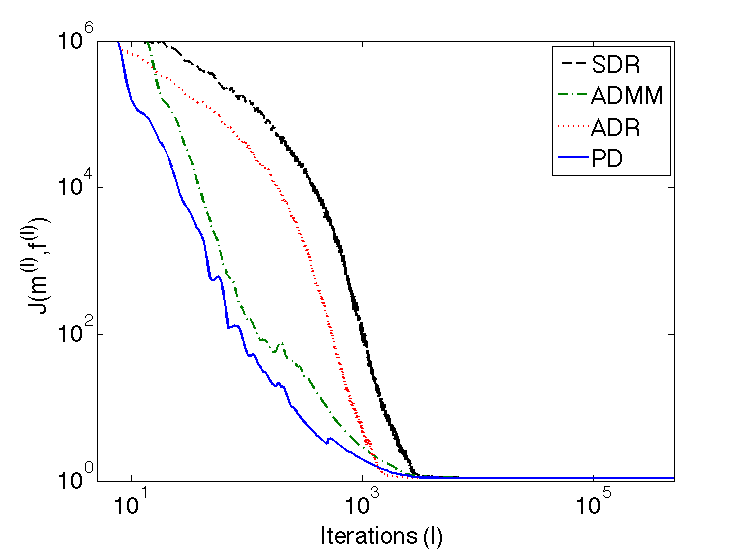
\includegraphics[trim=30 10 40 20,clip,width=0.33\textwidth]{images/J}&\hspace{-0.5cm}
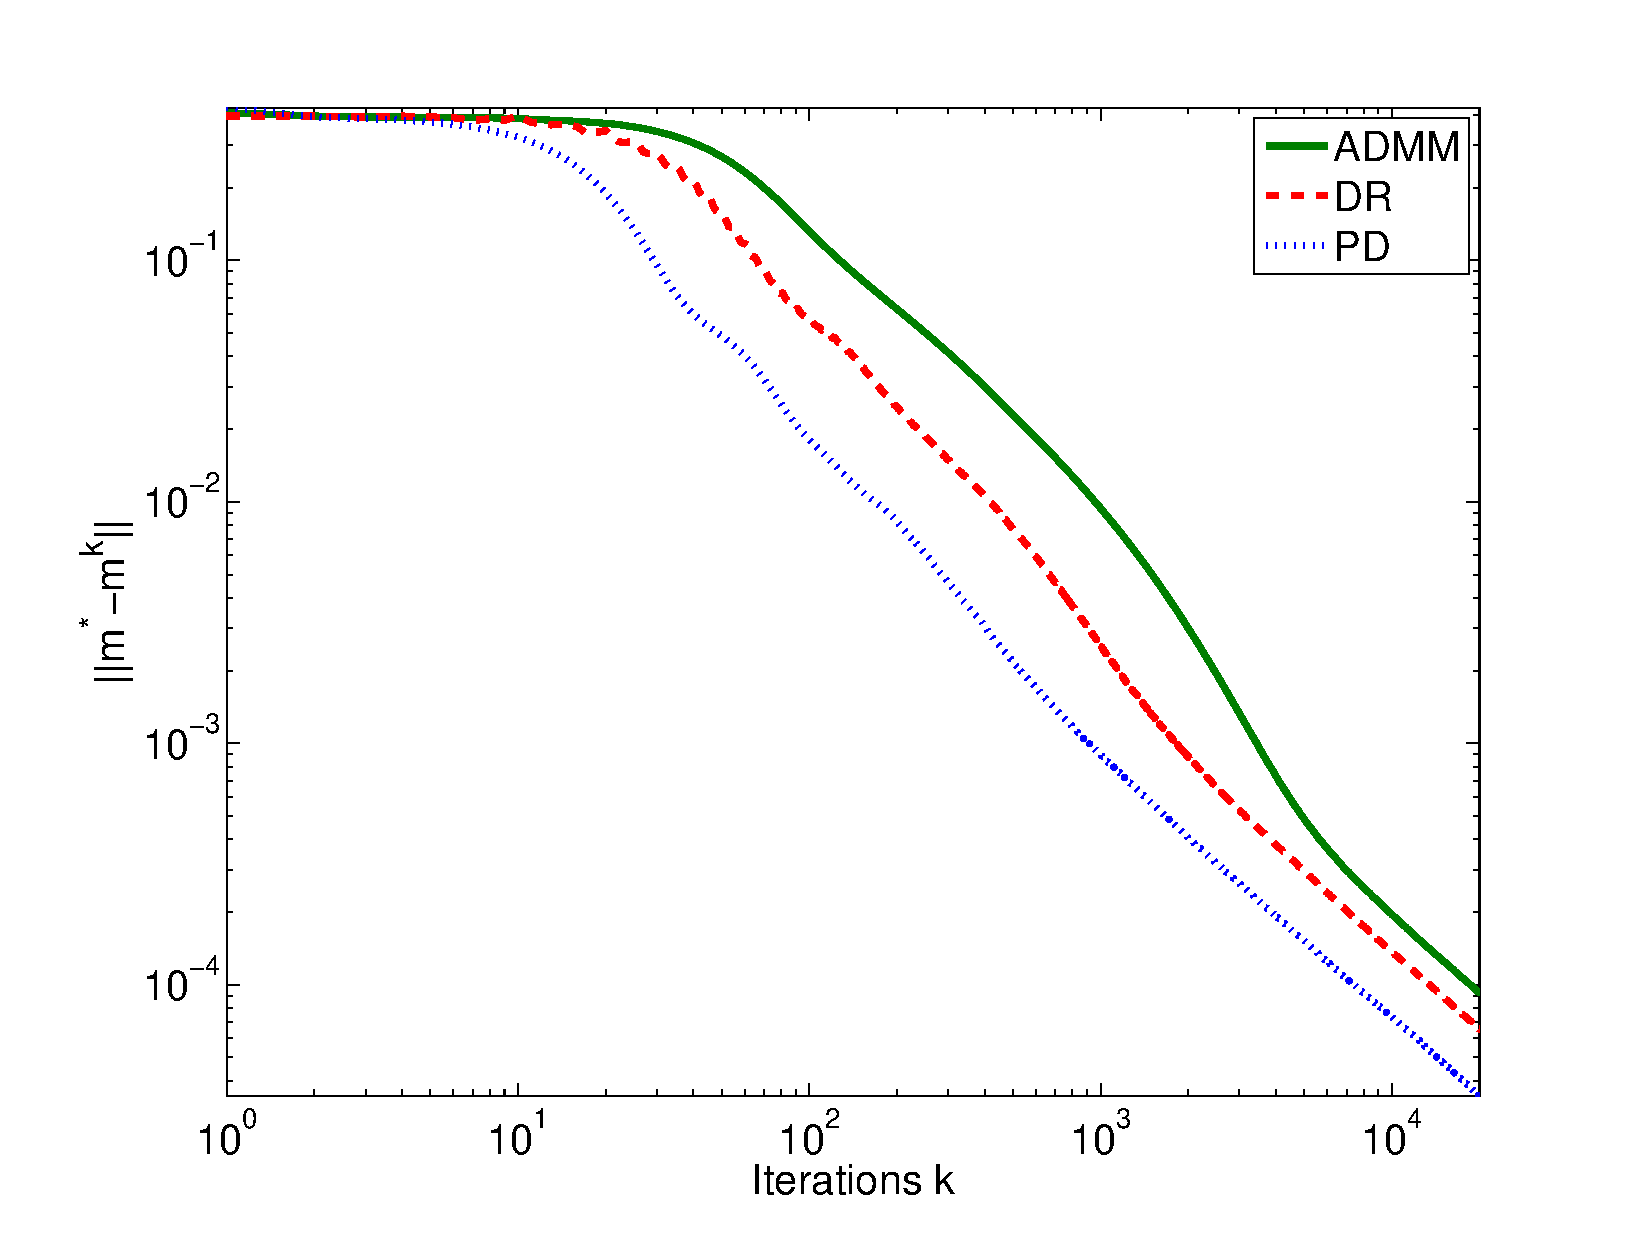
\includegraphics[trim=30 10 40 20,clip,width=0.33\textwidth]{images/convergence_m}&\hspace{-0.5cm}
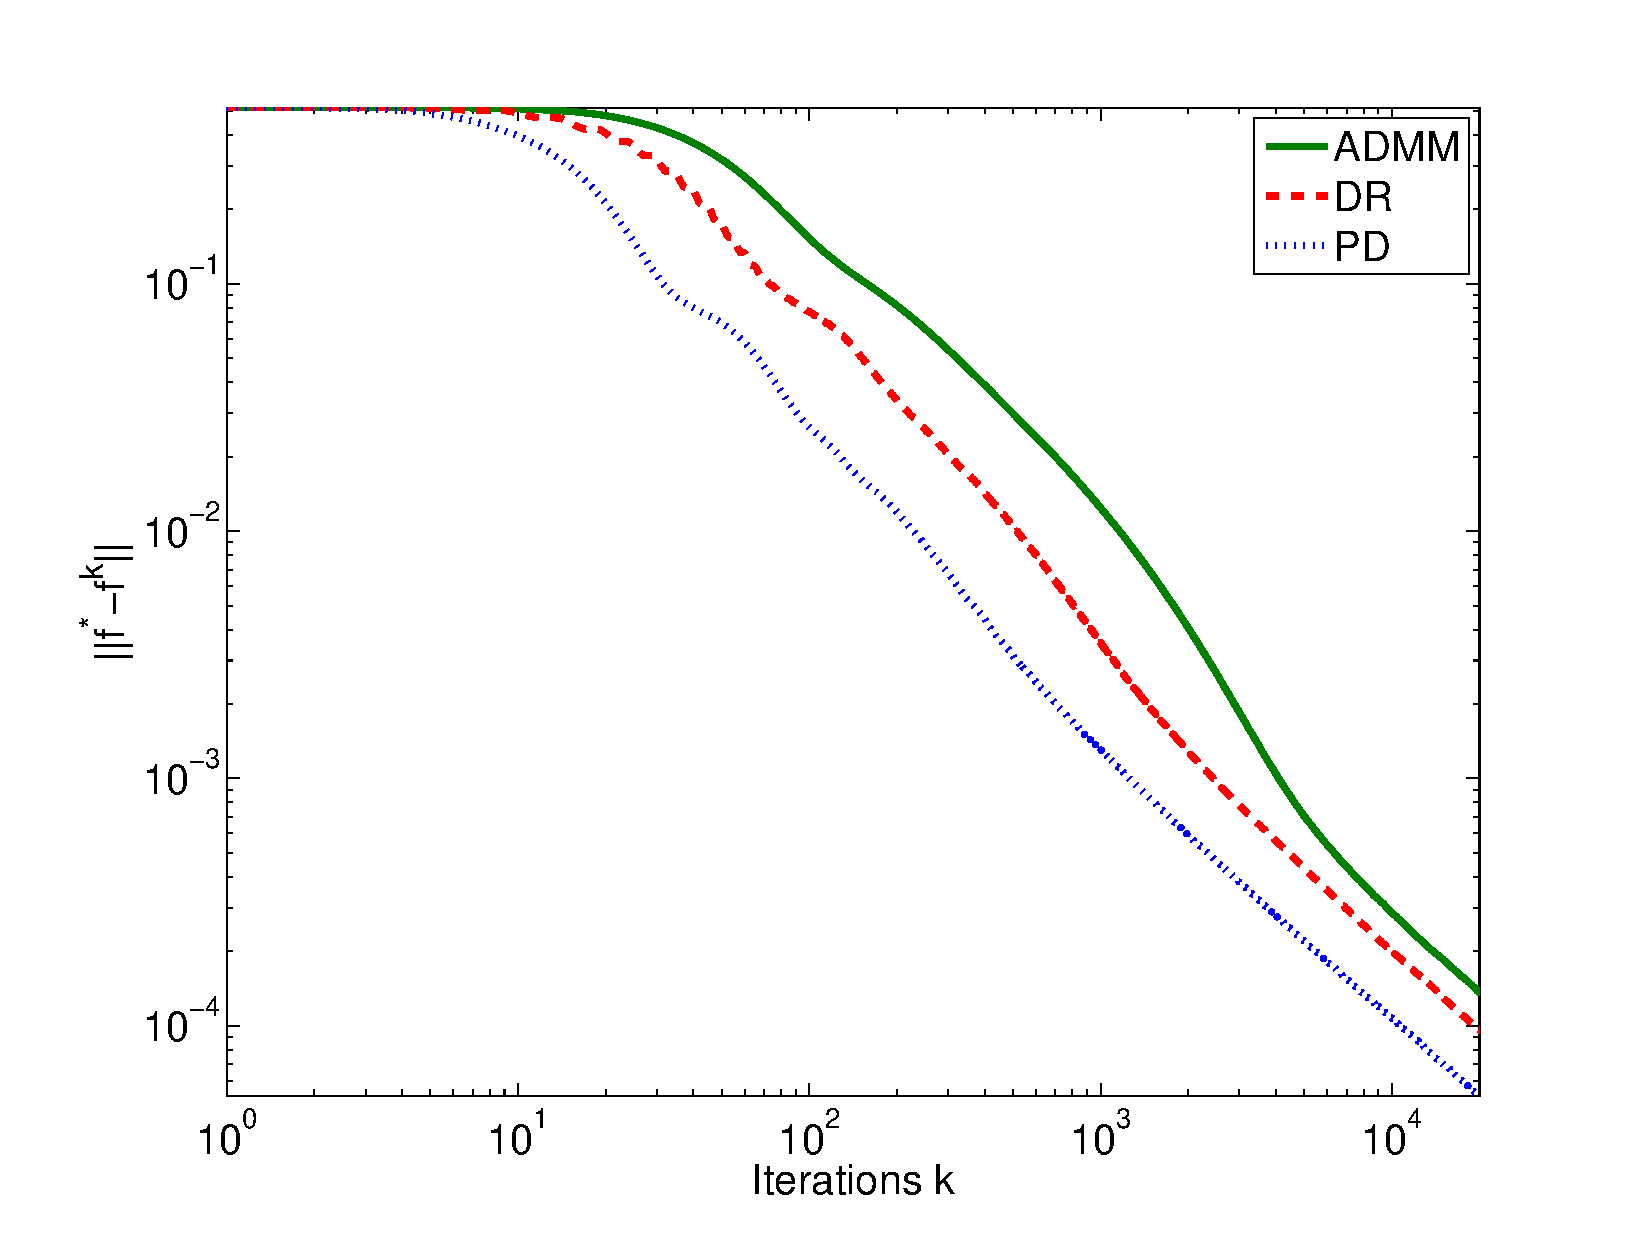
\includegraphics[trim=30 10 40 20,clip,width=0.33\textwidth]{images/convergence_f}\vspace{0.1cm}\\
$\Jfunc( \iter{m}, \iter{f} )$&\hspace{-0.5cm}$ \norm{m^\star-\iter{m}}$ &\hspace{-0.5cm}$ \norm{f^\star-\iter{f}}$ \vspace{-0.2cm}
\end{tabular}
\caption{\label{fig:comp_bump} 
	At each iteration $\ell$, we plot the value of the cost function $\Jfunc$ and the distance between the reference solution $(m^\star,f^\star)$ and the estimation $(\iter{m},\iter{f})$ for the different proximal splitting algorithms with the best found parameters. }
\end{center}
\end{figure}

When comparing the three approaches, PD presents the fastest convergence rate to the reference solution and the relaxed DR algorithm performs better than ADDM on the dual, which shows the advantage of introducing the $\al$ parameter. Note also that the computational cost is smaller for PD, as it takes\footnote{For our Matlab implementation on a standard laptop computer.} $0.13$s for one PD iteration and $0.2s$ for one DR or ADMM iteration for this example. 

% It can also  be noticed that PD is easier to parameterize. Indeed,  from the necessary relation $\sigma \tau \norm{\interp}^2<1$, one can chose $\si$ and then automatically fix $\tau=\frac{0.99}{\si \norm{\interp}^2}$. The exhaustive search has been realized in this way, thus involving a limited set of possible parameters for PD.




%%%%%%%%%%%%%%%%%%%%%%%%%%%%%%%%%%%%%%%%%%%%%%%%%%%%%%%%%%%%%%%%
%%%%%%%%%%%%%%%%%%%%%%%%%%%%%%%%%%%%%%%%%%%%%%%%%%%%%%%%%%%%%%%%
%%%%%%%%%%%%%%%%%%%%%%%%%%%%%%%%%%%%%%%%%%%%%%%%%%%%%%%%%%%%%%%%
\subsection{Interpolation Between $L^2$-Wasserstein and $H^{-1}$}

% Gabriel :  Wich $\ell$ is used ?

We first apply the PD algorithm for different values of $\beta$ on the bump example introduced in the previous section. The results are presented in the Figure~\ref{fig:generalized_bump}, which shows the level-lines of the estimated densities $\iter{f}(\cdot,t)$ for $\ell=1000$ iterations. It shows the evolution of the solution between a $H^{-1}$ linear interpolation ($\beta=0$) and a displacement interpolation with transport ($\beta=1$). 

% Gabriel : Ceci n'est pas terrible !! Essayer de le corriger ?
% Nicolas: Corrig�

% Notice that the minimum value of $f^0$ and $f^1$ has been bounded with the value $10^{-8}$, so that the true transport is not exactly a translation for the case $\beta=1$. This explains the slight deformations of the circles in the last line of Figure \ref{fig:generalized_bump}. 


\newcommand{\sidecap}[1]{ {\begin{sideways}\parbox{1.6cm}{\centering #1}\end{sideways}} }
\begin{figure}[!ht]
\begin{center}
\begin{tabular}{cccccccccc}
\sidecap{$\beta=0$ } &\hspace{-0.45cm}
%\animategraphics[palindrome=true,width=1.6cm]{6}{images/bump_anim/bump_beta_0_iso_}{01}{33}&
%\movie[mouse=true,palindrome=true]{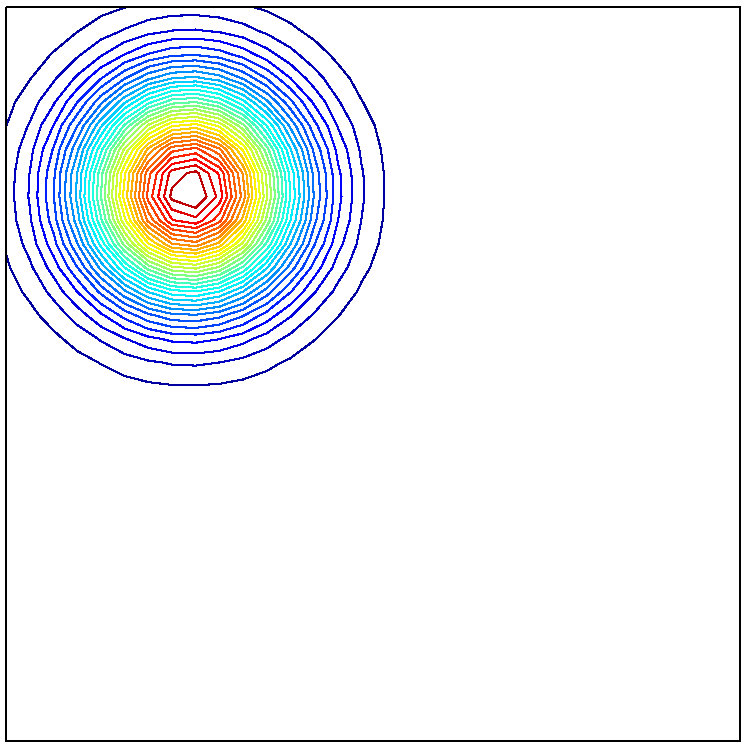
\includegraphics[width=1.6cm]{images/bump_beta/bump_beta_0_iso_01}}{images/bump_beta/beta_0.avi}&
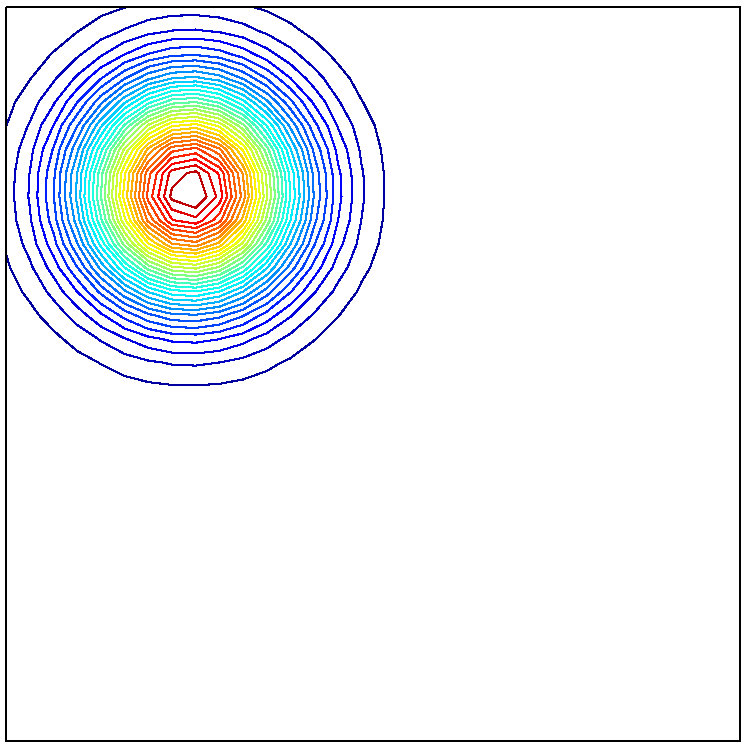
\includegraphics[width=1.6cm]{images/bump_beta/bump_beta_0_iso_01}&
\hspace{-0.45cm}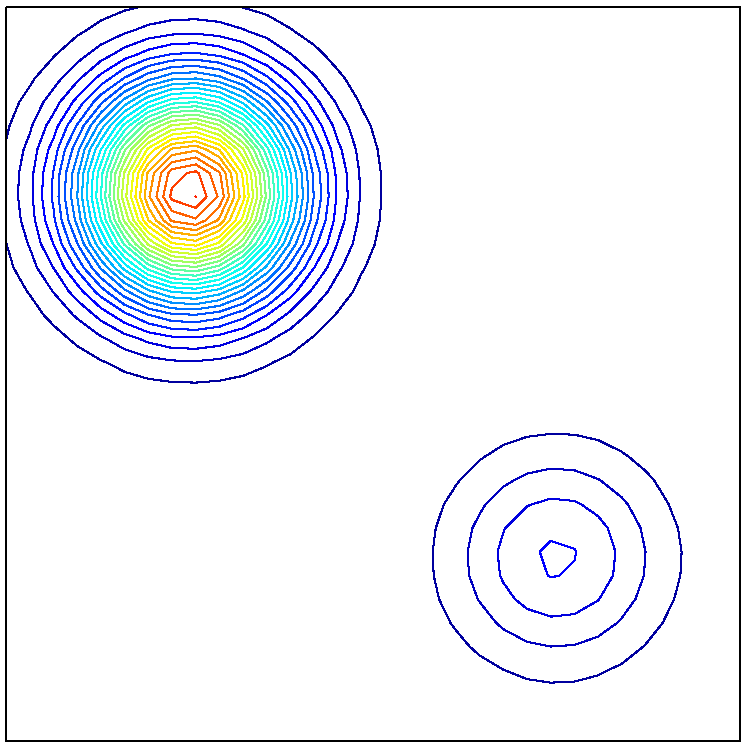
\includegraphics[width=1.6cm]{images/bump_beta/bump_beta_0_iso_05}&
\hspace{-0.45cm}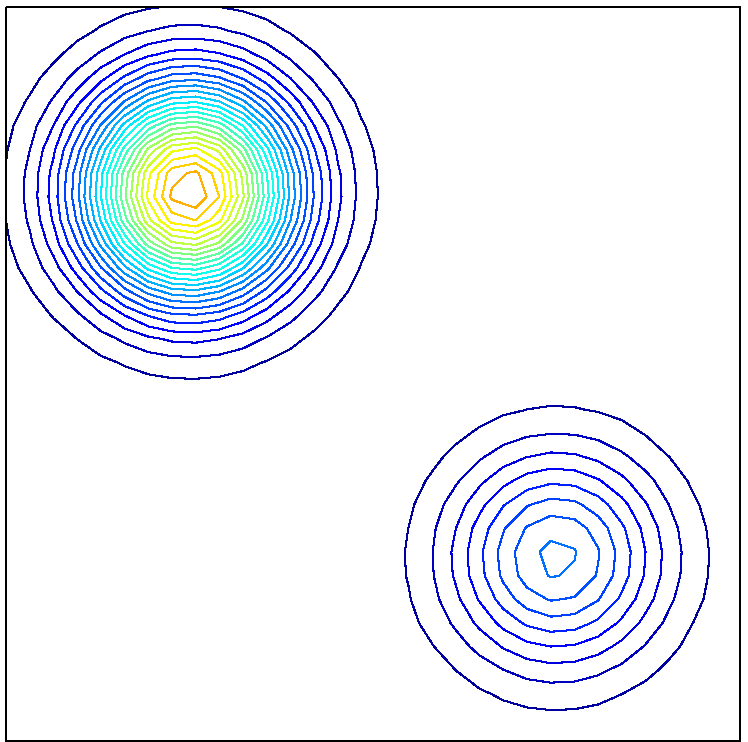
\includegraphics[width=1.6cm]{images/bump_beta/bump_beta_0_iso_09}&
\hspace{-0.45cm}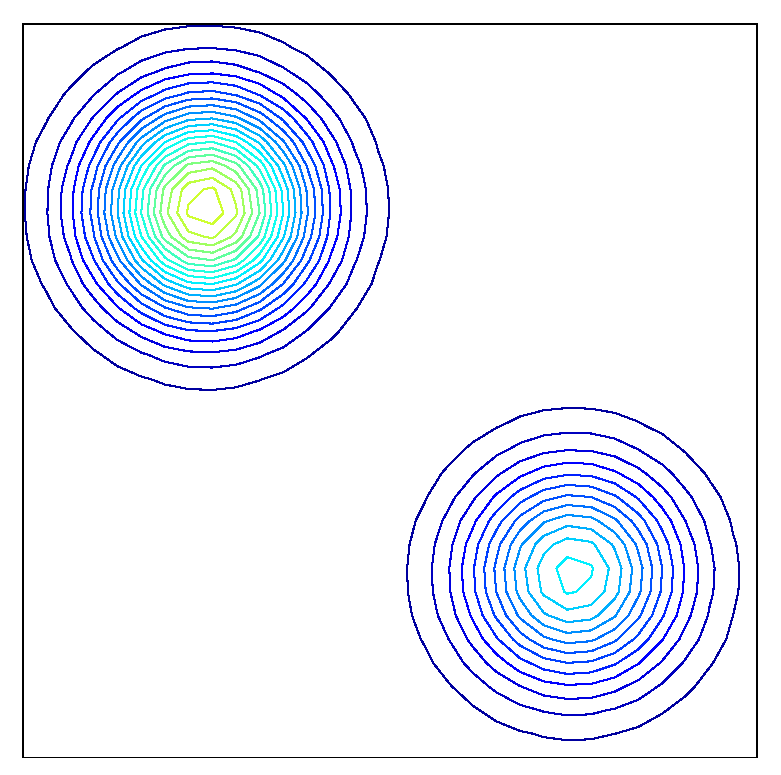
\includegraphics[width=1.6cm]{images/bump_beta/bump_beta_0_iso_13}&
\hspace{-0.45cm}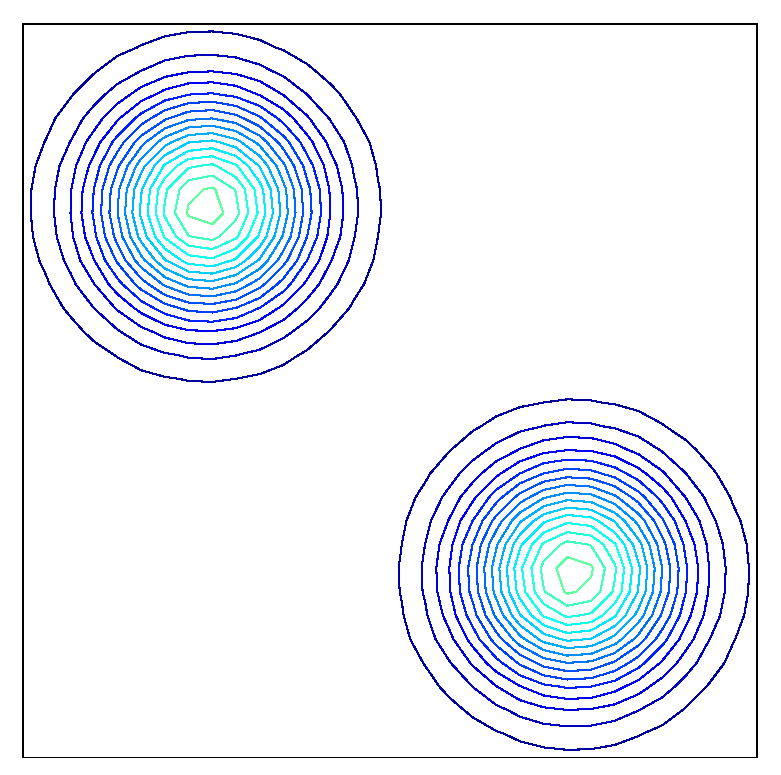
\includegraphics[width=1.6cm]{images/bump_beta/bump_beta_0_iso_17}&
\hspace{-0.45cm}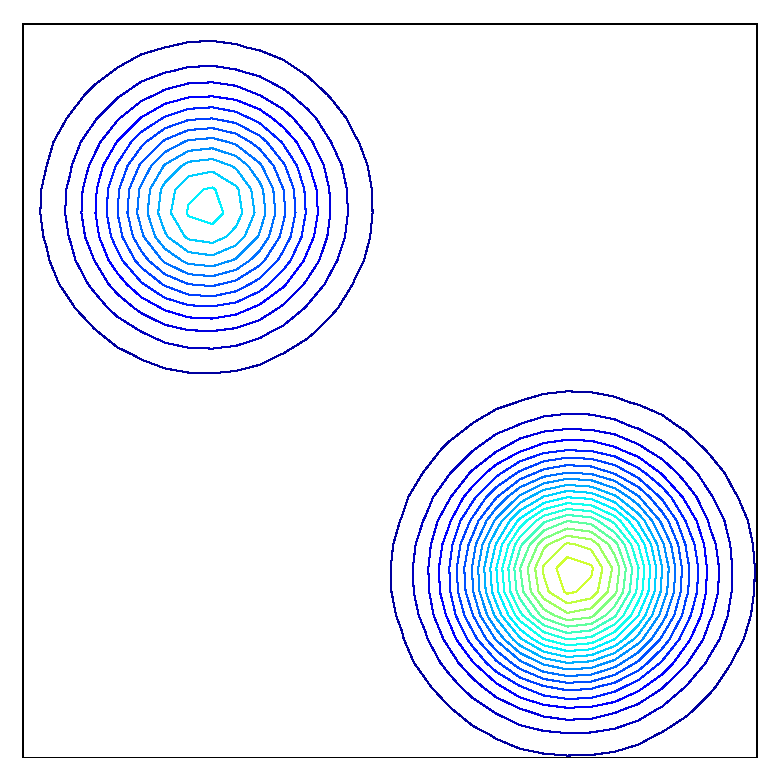
\includegraphics[width=1.6cm]{images/bump_beta/bump_beta_0_iso_21}&
\hspace{-0.45cm}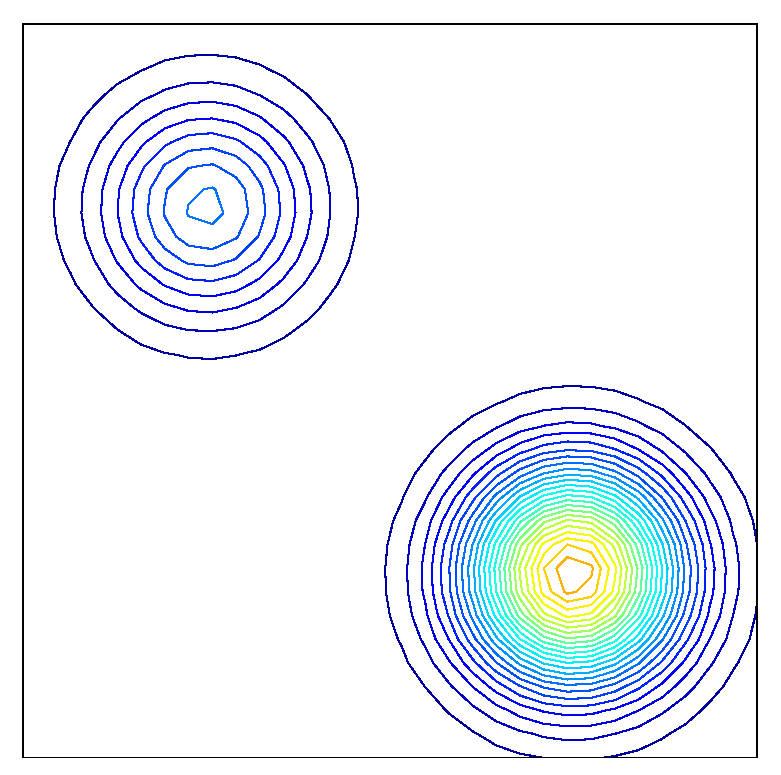
\includegraphics[width=1.6cm]{images/bump_beta/bump_beta_0_iso_25}&
\hspace{-0.45cm}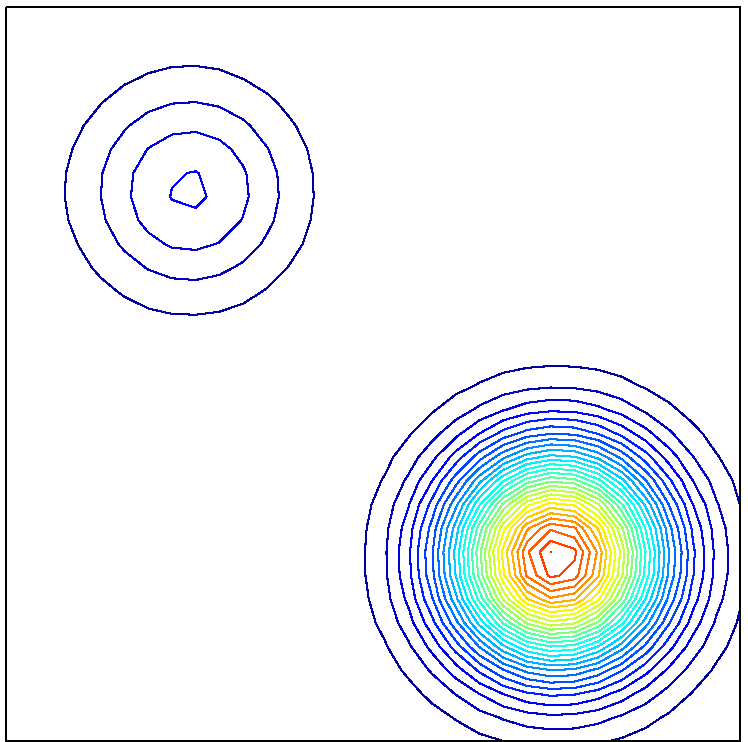
\includegraphics[width=1.6cm]{images/bump_beta/bump_beta_0_iso_29}&
\hspace{-0.45cm}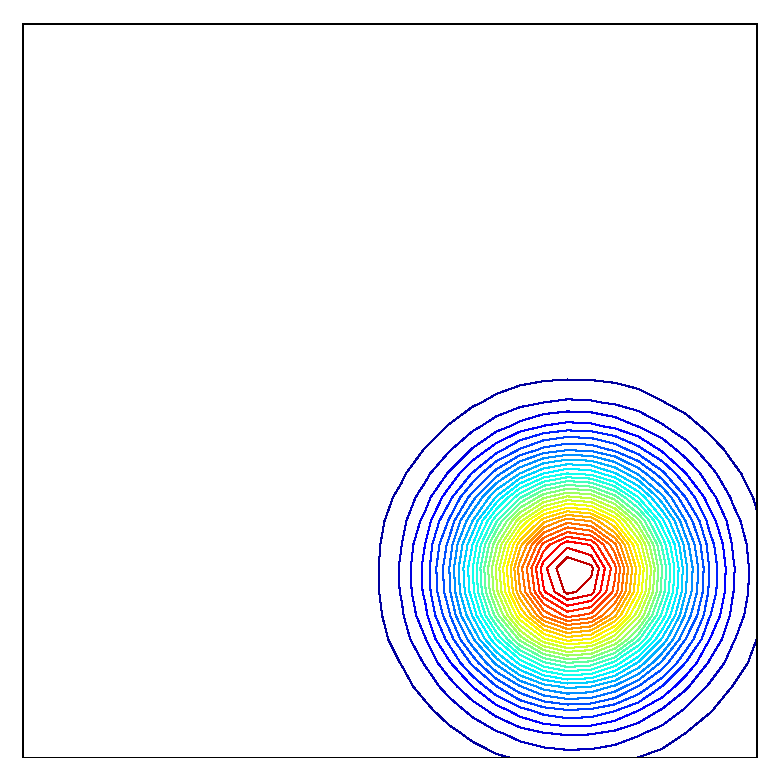
\includegraphics[width=1.6cm]{images/bump_beta/bump_beta_0_iso_33}\\
\sidecap{$\beta=1/4$ } &\hspace{-0.45cm}
%\animategraphics[palindrome=true,width=1.6cm]{6}{images/bump_anim/bump_beta_25_iso_}{01}{33}&
%\movie[mouse=true,palindrome=true]{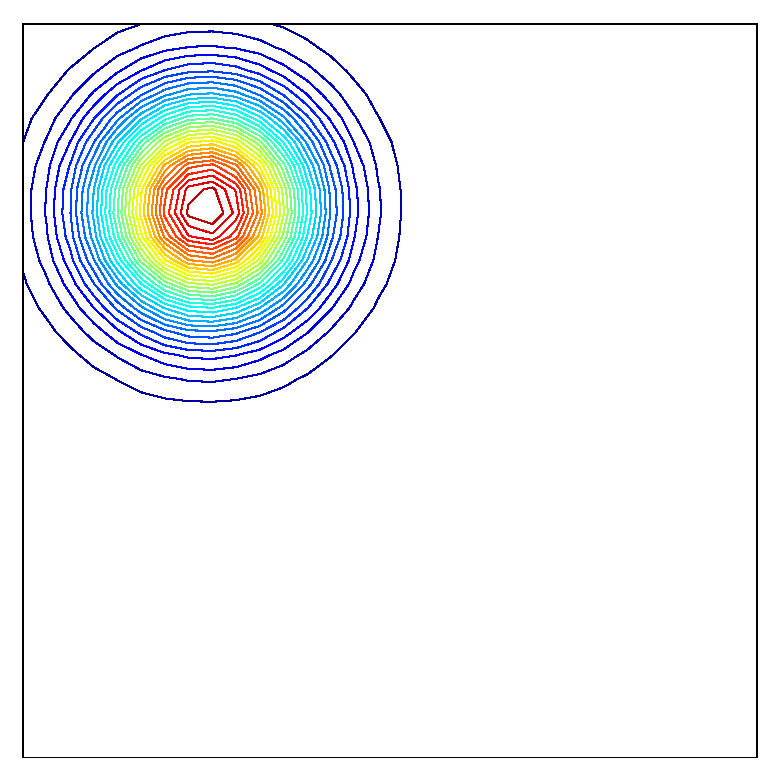
\includegraphics[width=1.6cm]{images/bump_beta/bump_beta_25_iso_01}}{images/bump_beta/beta_25.avi}&
%
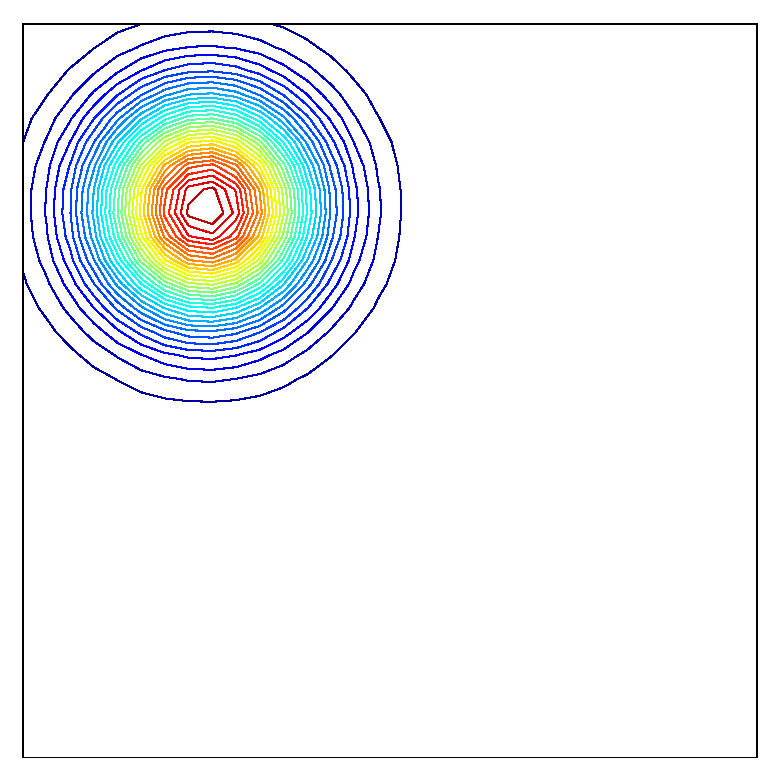
\includegraphics[width=1.6cm]{images/bump_beta/bump_beta_25_iso_01}&
\hspace{-0.45cm}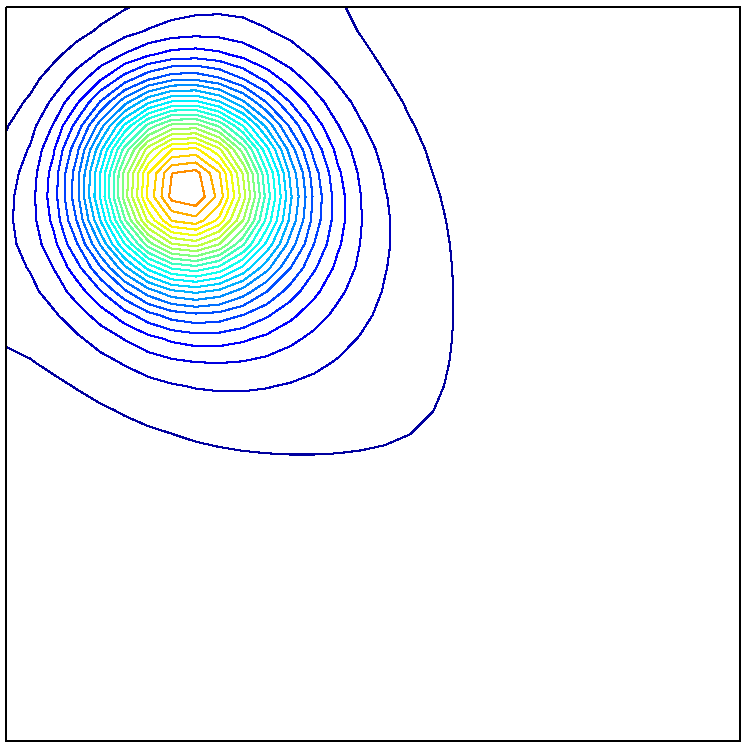
\includegraphics[width=1.6cm]{images/bump_beta/bump_beta_25_iso_05}&
\hspace{-0.45cm}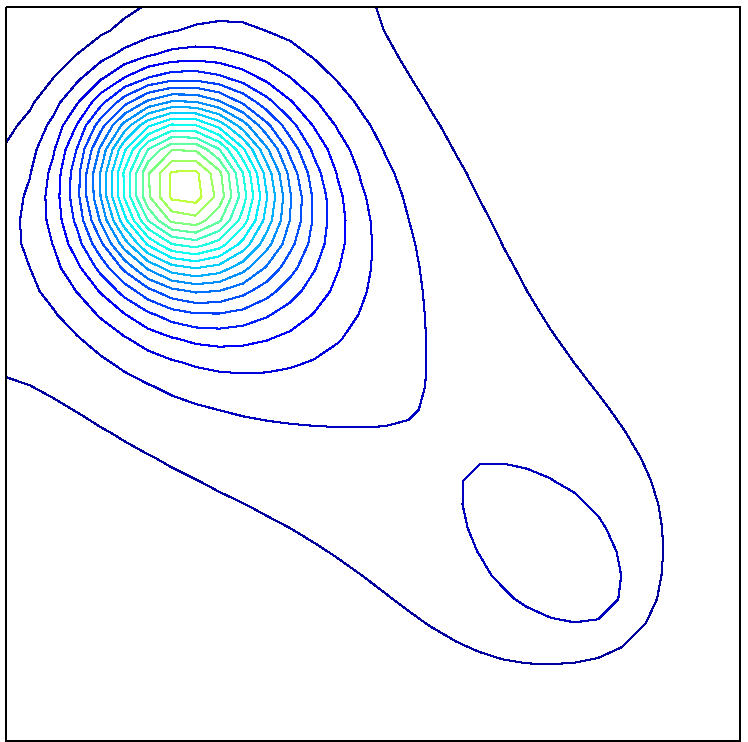
\includegraphics[width=1.6cm]{images/bump_beta/bump_beta_25_iso_09}&
\hspace{-0.45cm}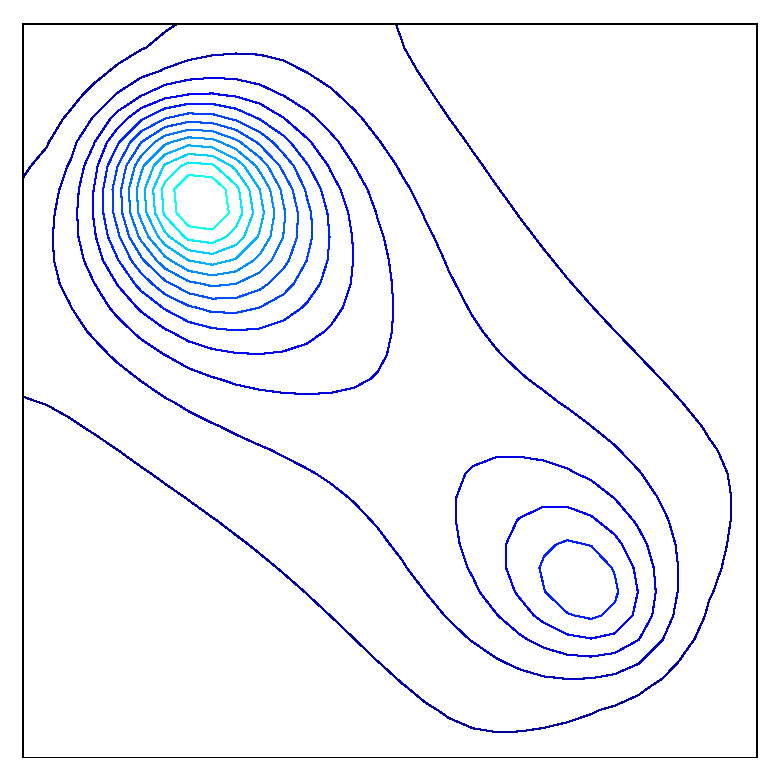
\includegraphics[width=1.6cm]{images/bump_beta/bump_beta_25_iso_13}&
\hspace{-0.45cm}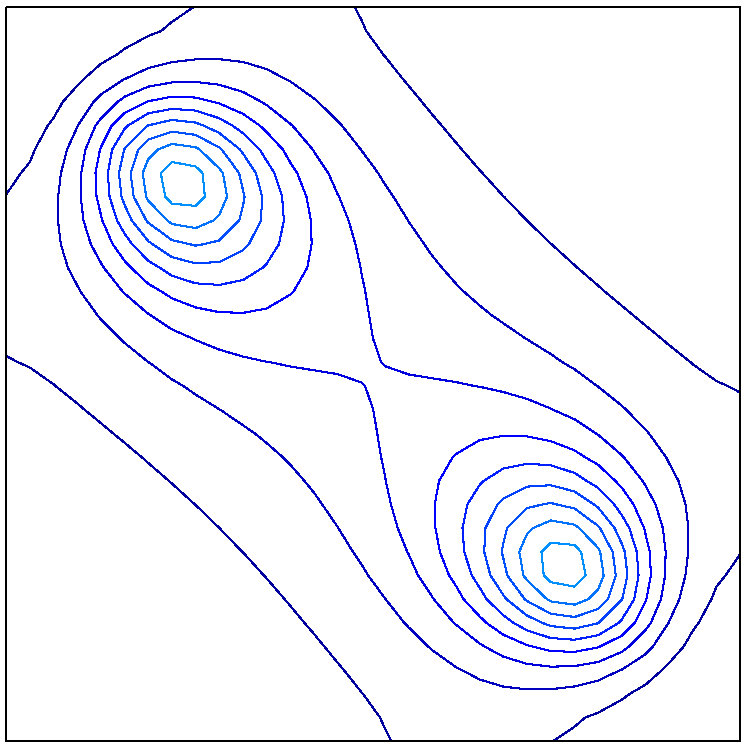
\includegraphics[width=1.6cm]{images/bump_beta/bump_beta_25_iso_17}&
\hspace{-0.45cm}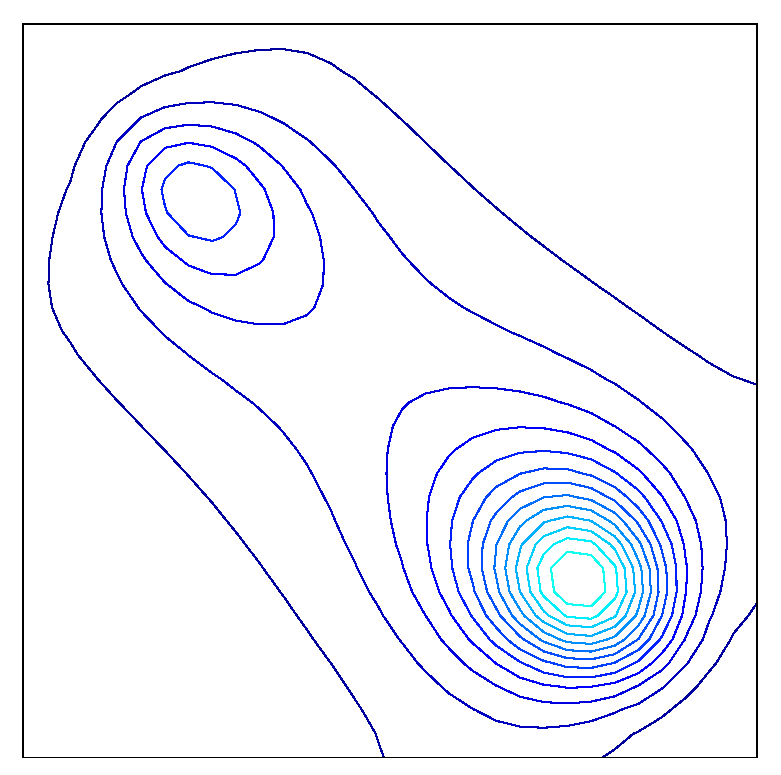
\includegraphics[width=1.6cm]{images/bump_beta/bump_beta_25_iso_21}&
\hspace{-0.45cm}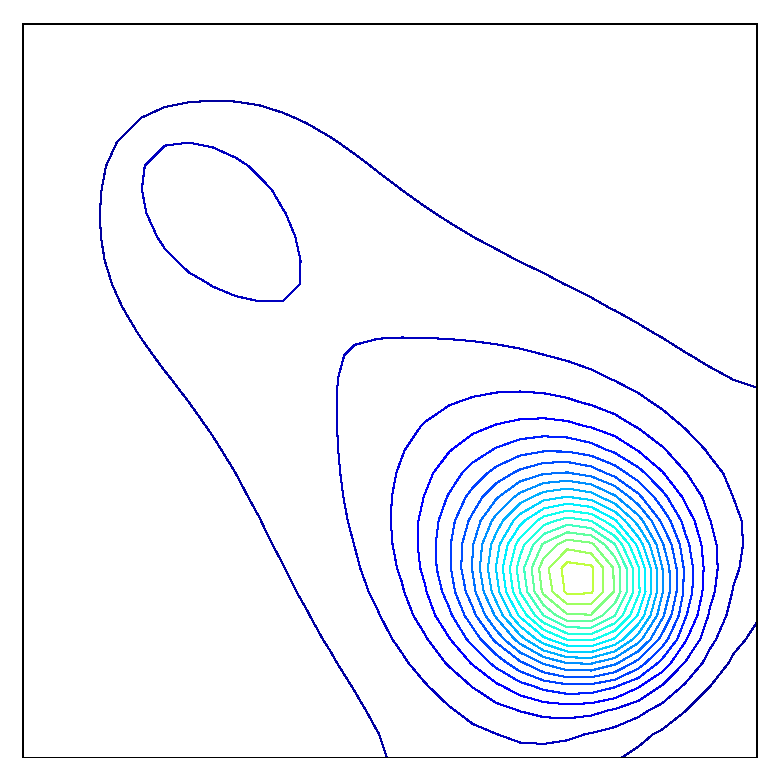
\includegraphics[width=1.6cm]{images/bump_beta/bump_beta_25_iso_25}&
\hspace{-0.45cm}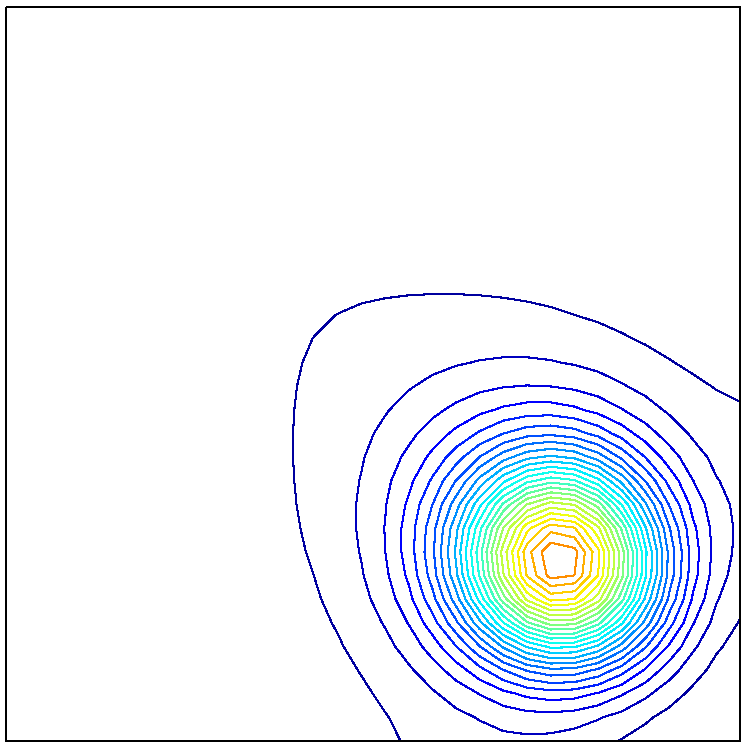
\includegraphics[width=1.6cm]{images/bump_beta/bump_beta_25_iso_29}&
\hspace{-0.45cm}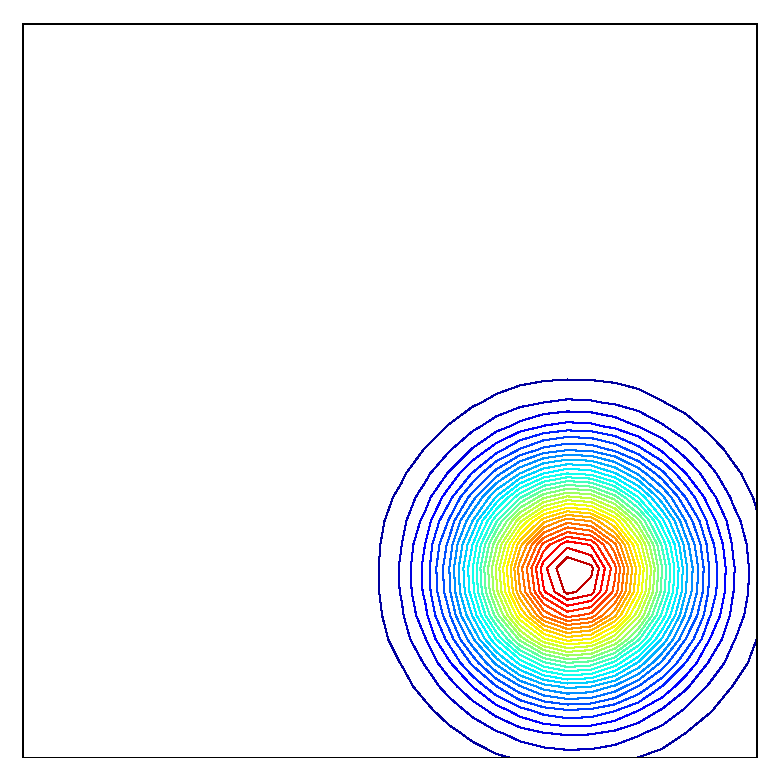
\includegraphics[width=1.6cm]{images/bump_beta/bump_beta_25_iso_33}\\
\sidecap{$\beta=1/2$ } &\hspace{-0.45cm}
%\animategraphics[palindrome=true,width=1.6cm]{6}{images/bump_anim/bump_beta_05_iso_}{01}{33}&
%\movie[mouse=true,palindrome=true]{\includegraphics[width=1.6cm]{images/bump_beta/bump_beta_05_iso_01}}{images/bump_beta/beta_05.avi}&
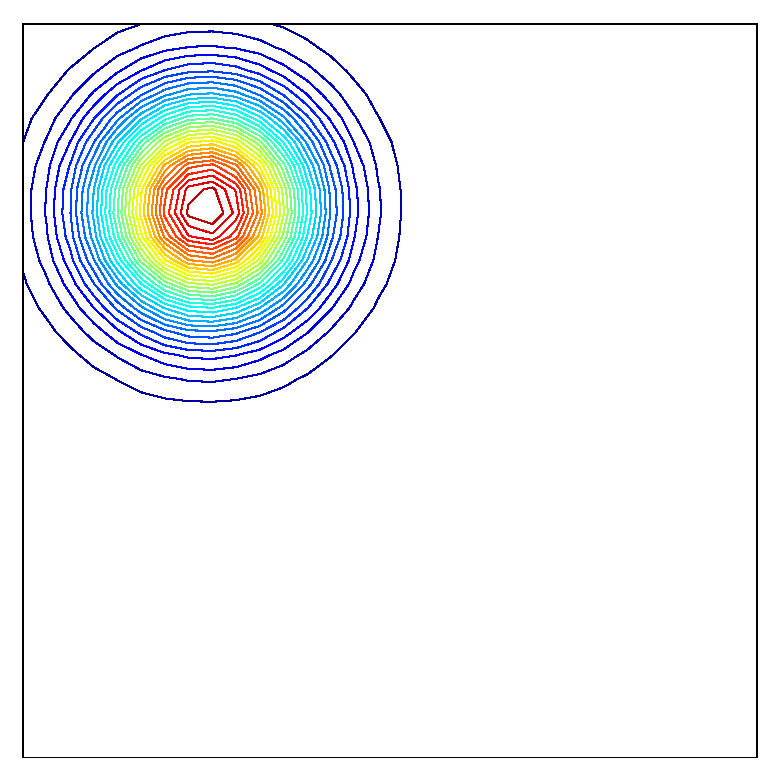
\includegraphics[width=1.6cm]{images/bump_beta/bump_beta_50_iso_01}&
\hspace{-0.45cm}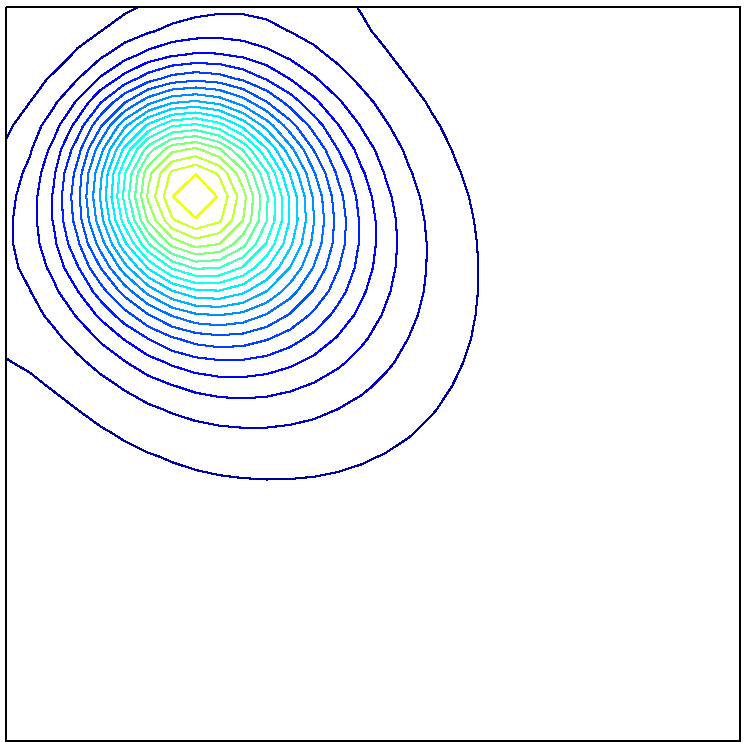
\includegraphics[width=1.6cm]{images/bump_beta/bump_beta_50_iso_05}&
\hspace{-0.45cm}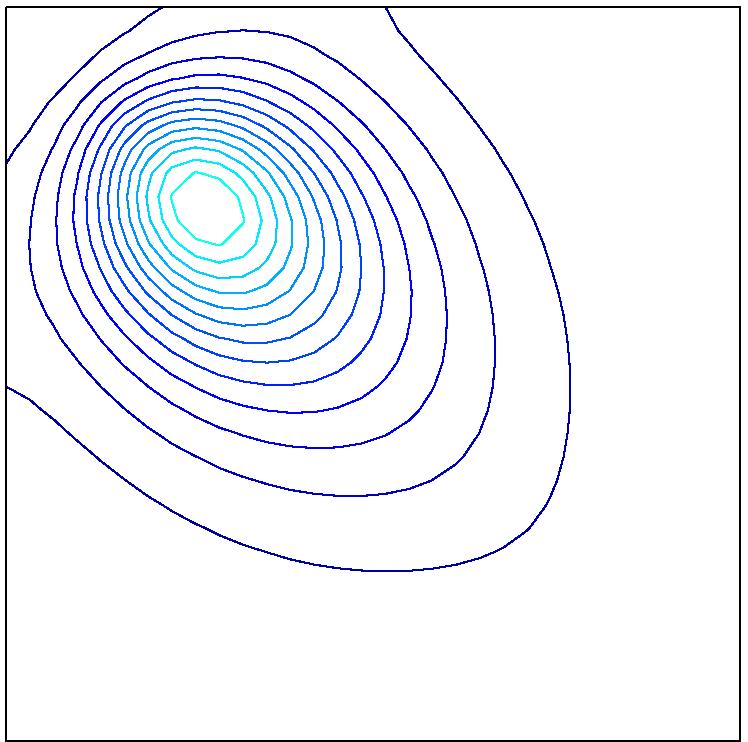
\includegraphics[width=1.6cm]{images/bump_beta/bump_beta_50_iso_09}&
\hspace{-0.45cm}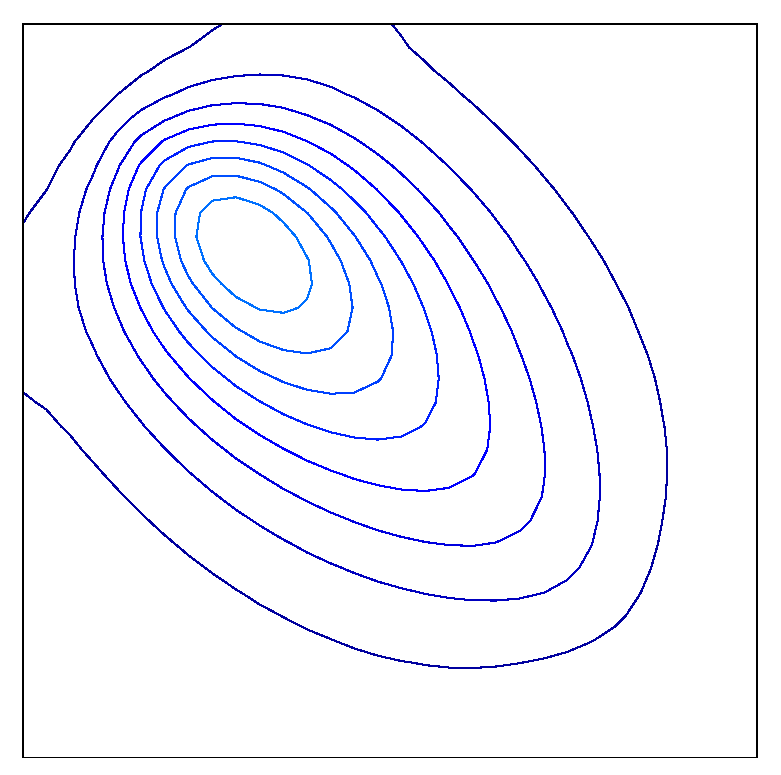
\includegraphics[width=1.6cm]{images/bump_beta/bump_beta_50_iso_13}&
\hspace{-0.45cm}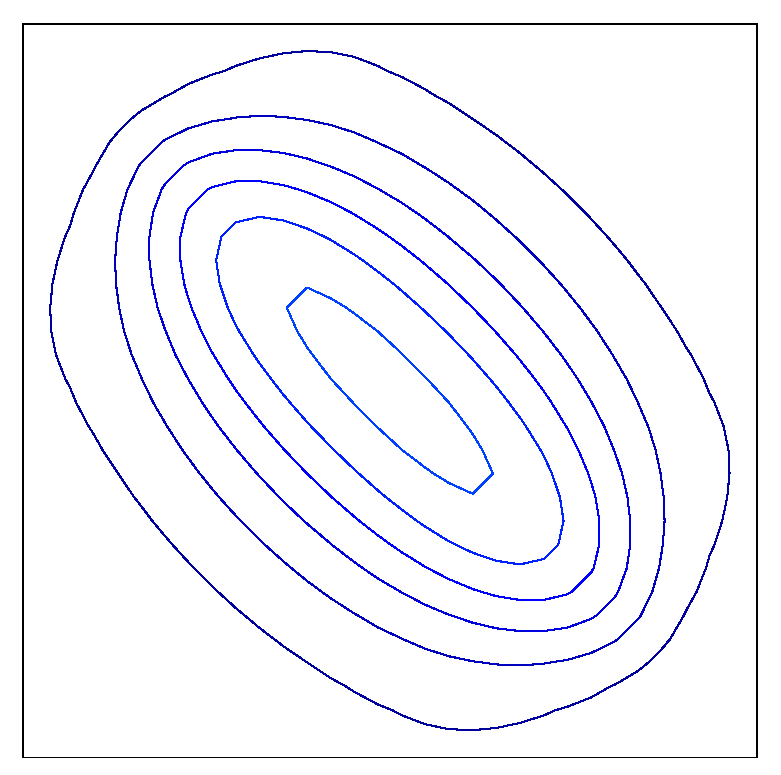
\includegraphics[width=1.6cm]{images/bump_beta/bump_beta_50_iso_17}&
\hspace{-0.45cm}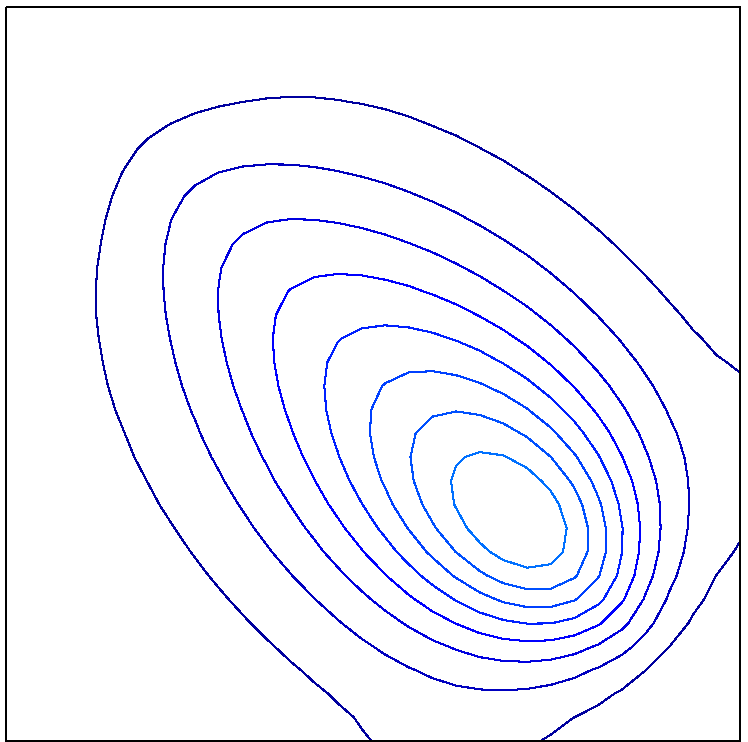
\includegraphics[width=1.6cm]{images/bump_beta/bump_beta_50_iso_21}&
\hspace{-0.45cm}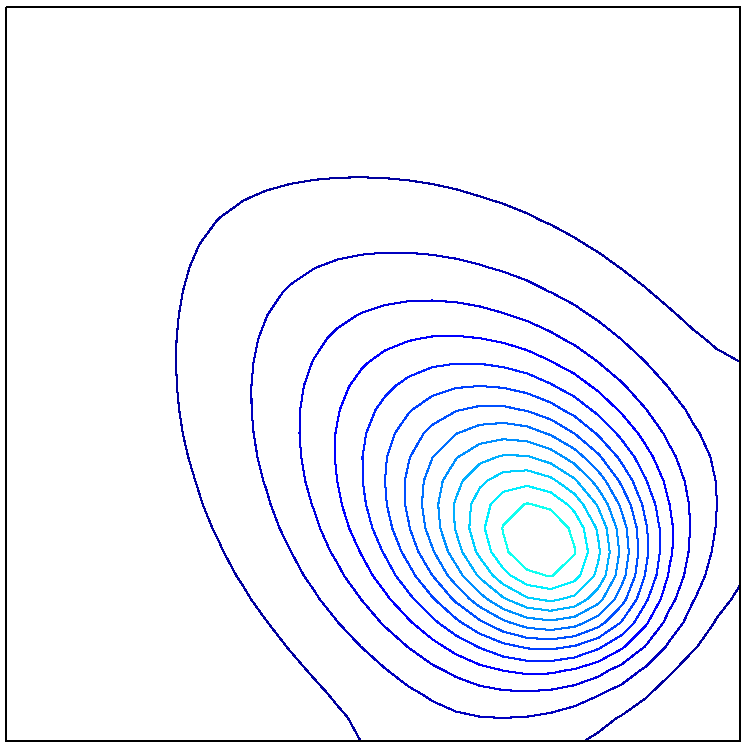
\includegraphics[width=1.6cm]{images/bump_beta/bump_beta_50_iso_25}&
\hspace{-0.45cm}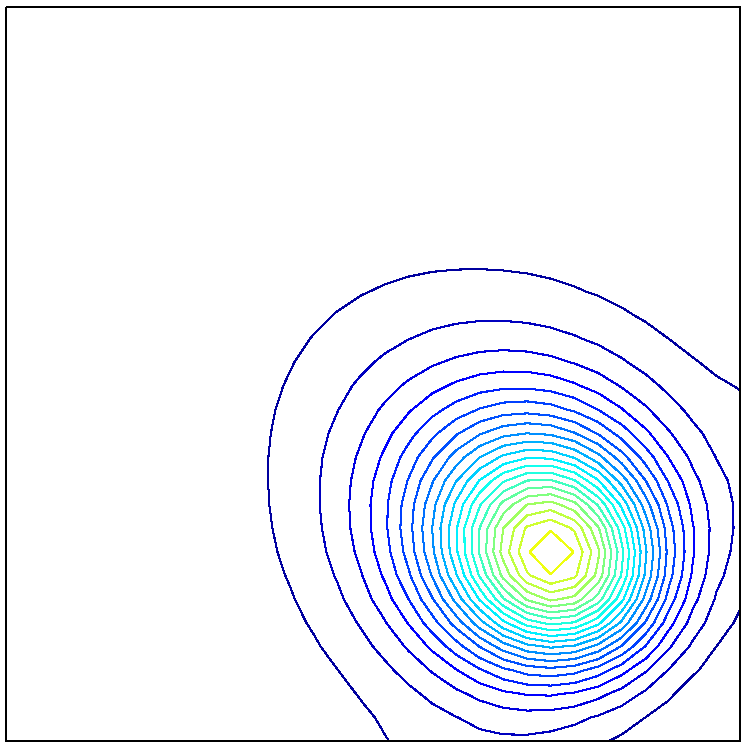
\includegraphics[width=1.6cm]{images/bump_beta/bump_beta_50_iso_29}&
\hspace{-0.45cm}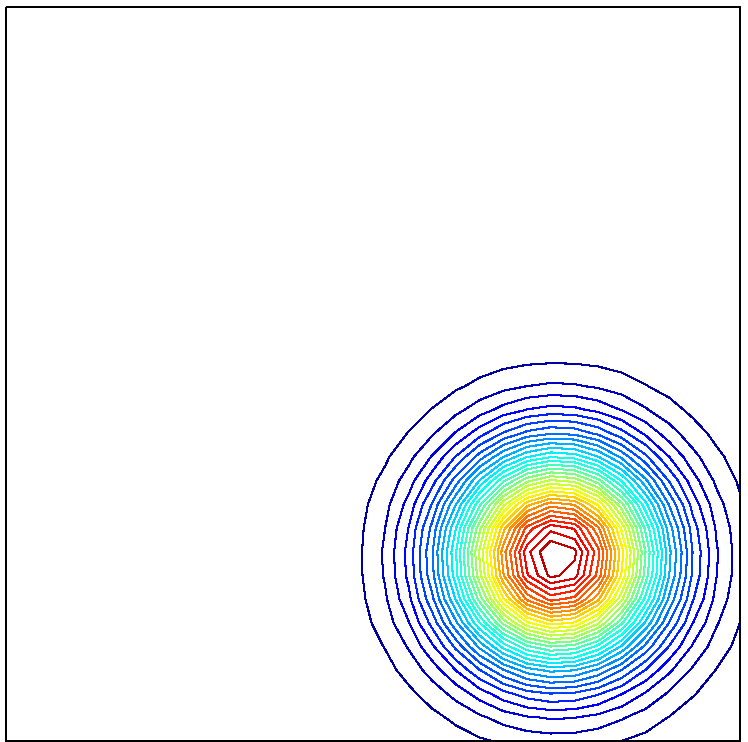
\includegraphics[width=1.6cm]{images/bump_beta/bump_beta_50_iso_33}\\
\sidecap{$\beta=3/4$ } &\hspace{-0.45cm}
%\animategraphics[palindrome=true,width=1.6cm]{6}{images/bump_anim/bump_beta_75_iso_}{01}{33}&
%\movie[mouse=true,palindrome=true]{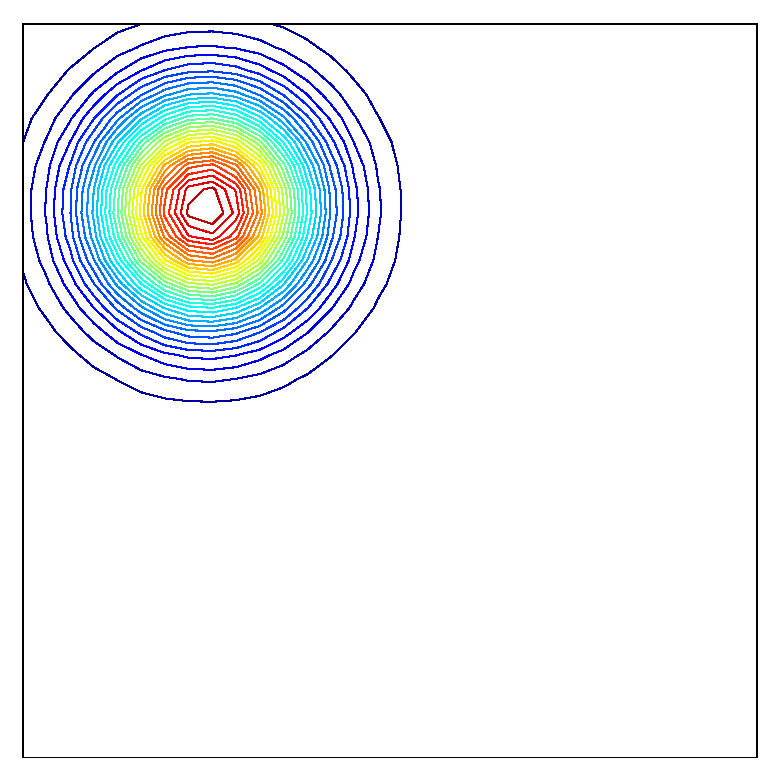
\includegraphics[width=1.6cm]{images/bump_beta/bump_beta_75_iso_01}}{images/bump_beta/beta_75.avi}&
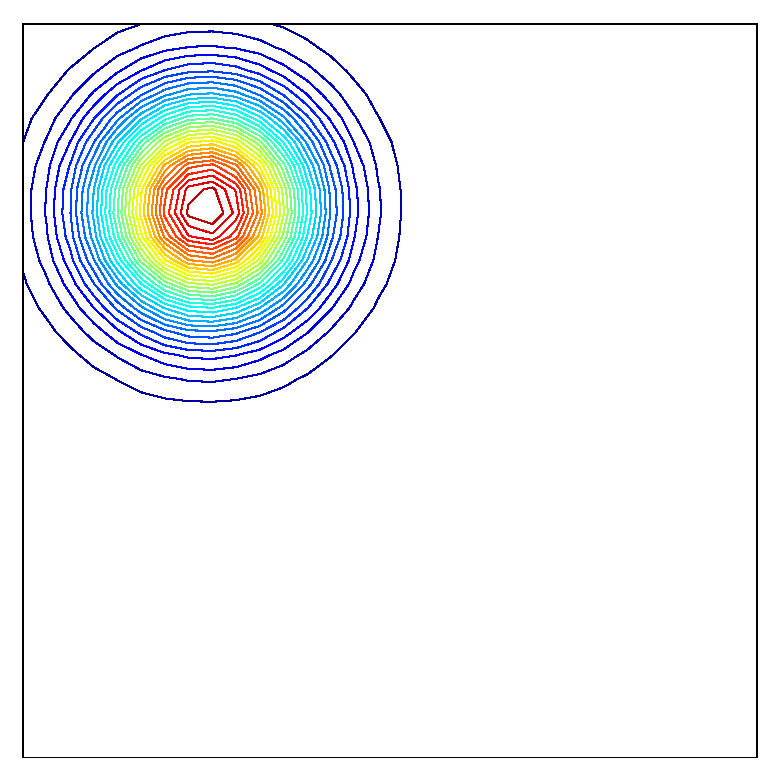
\includegraphics[width=1.6cm]{images/bump_beta/bump_beta_75_iso_01}&
\hspace{-0.45cm}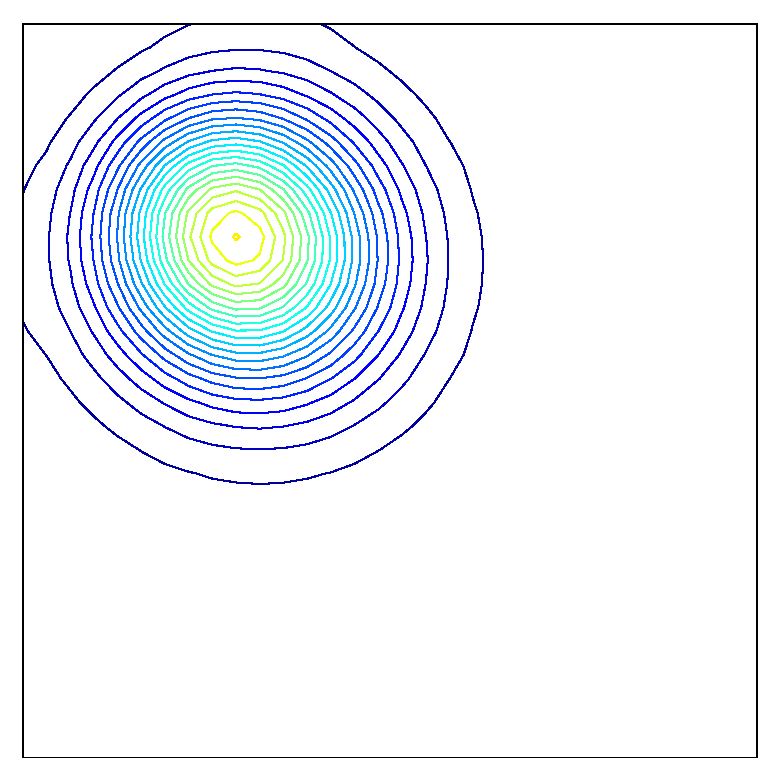
\includegraphics[width=1.6cm]{images/bump_beta/bump_beta_75_iso_05}&
\hspace{-0.45cm}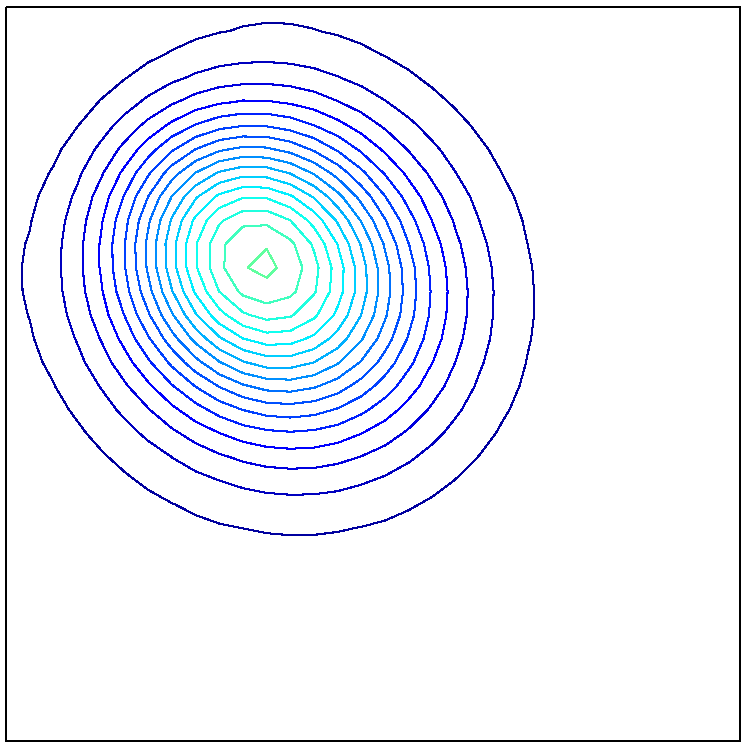
\includegraphics[width=1.6cm]{images/bump_beta/bump_beta_75_iso_09}&
\hspace{-0.45cm}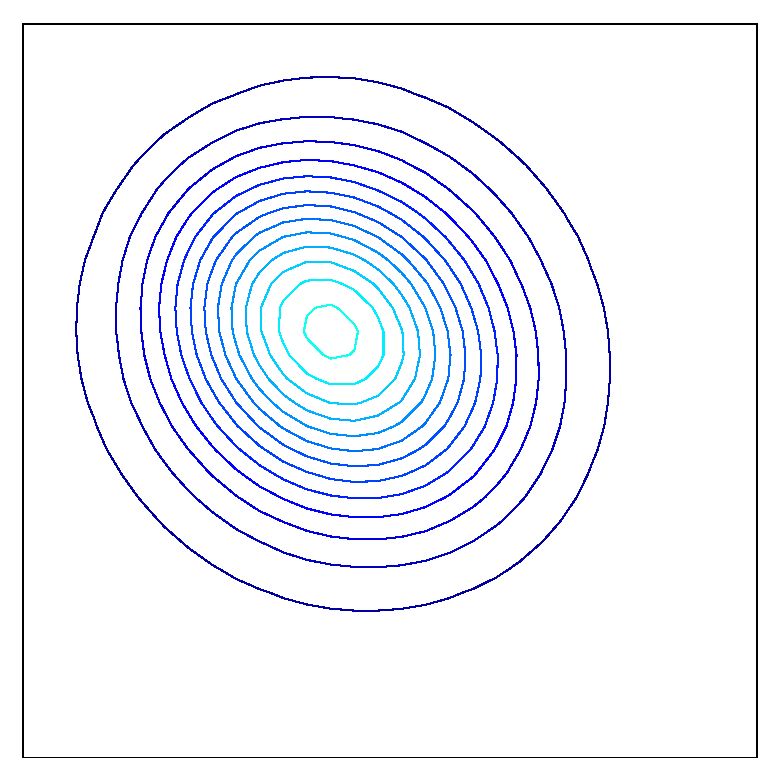
\includegraphics[width=1.6cm]{images/bump_beta/bump_beta_75_iso_13}&
\hspace{-0.45cm}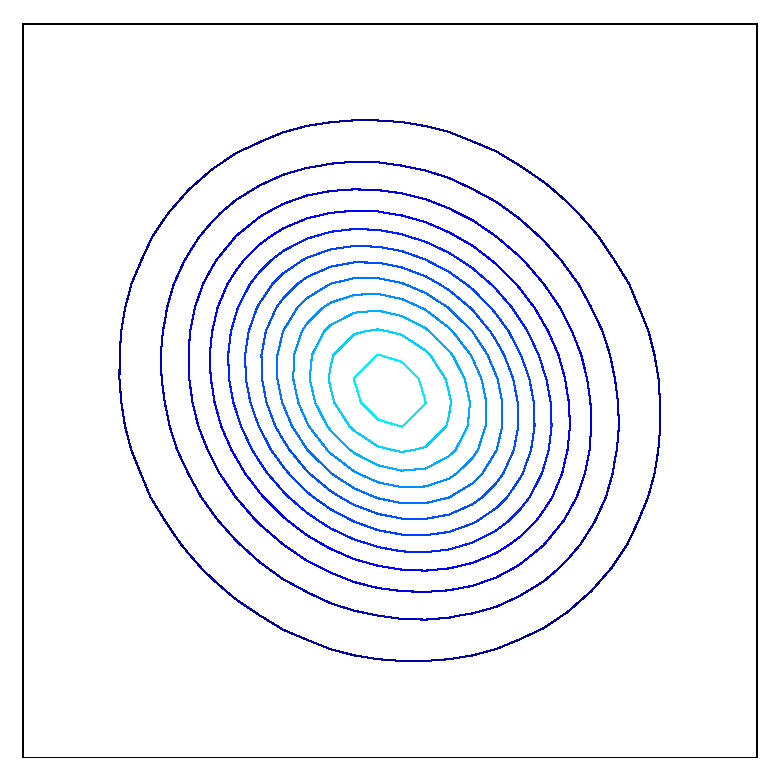
\includegraphics[width=1.6cm]{images/bump_beta/bump_beta_75_iso_17}&
\hspace{-0.45cm}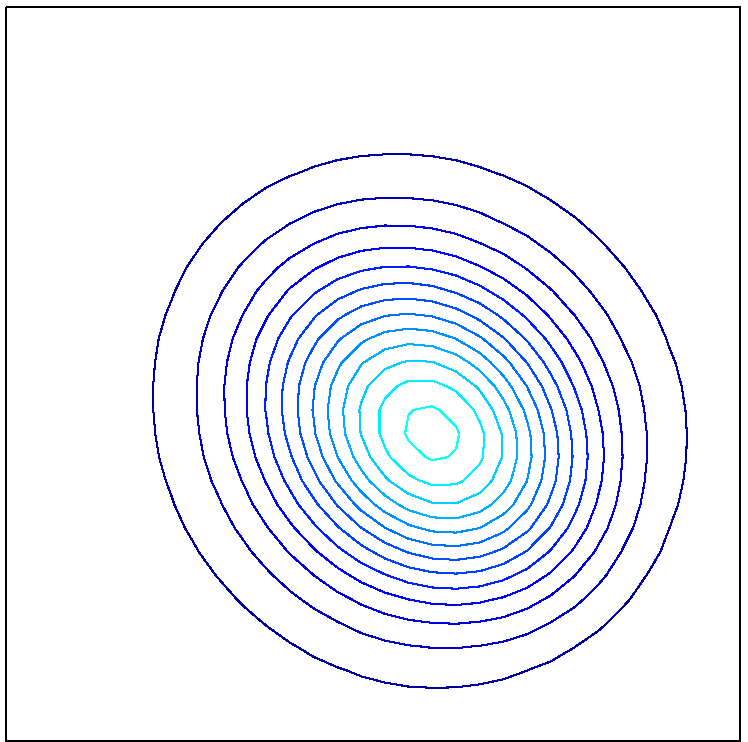
\includegraphics[width=1.6cm]{images/bump_beta/bump_beta_75_iso_21}&
\hspace{-0.45cm}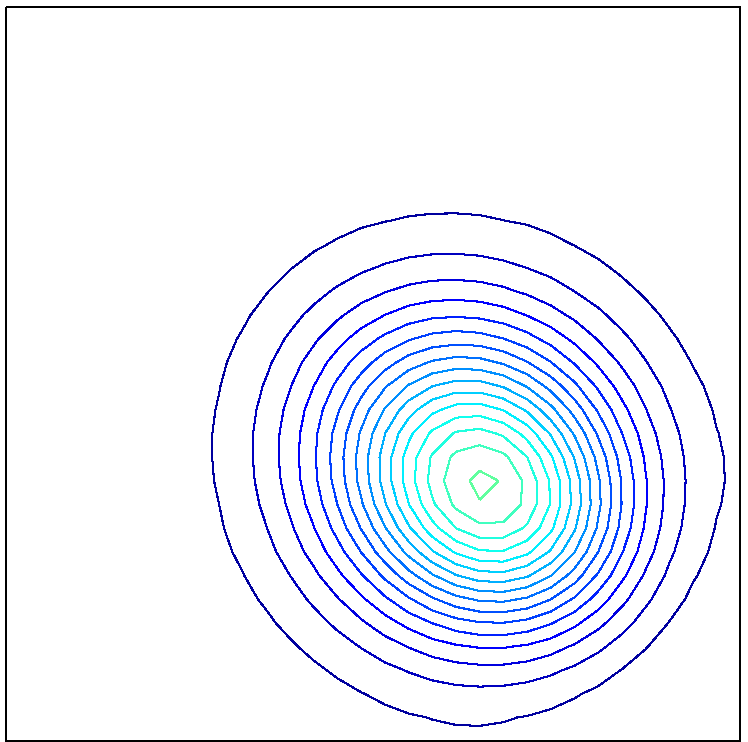
\includegraphics[width=1.6cm]{images/bump_beta/bump_beta_75_iso_25}&
\hspace{-0.45cm}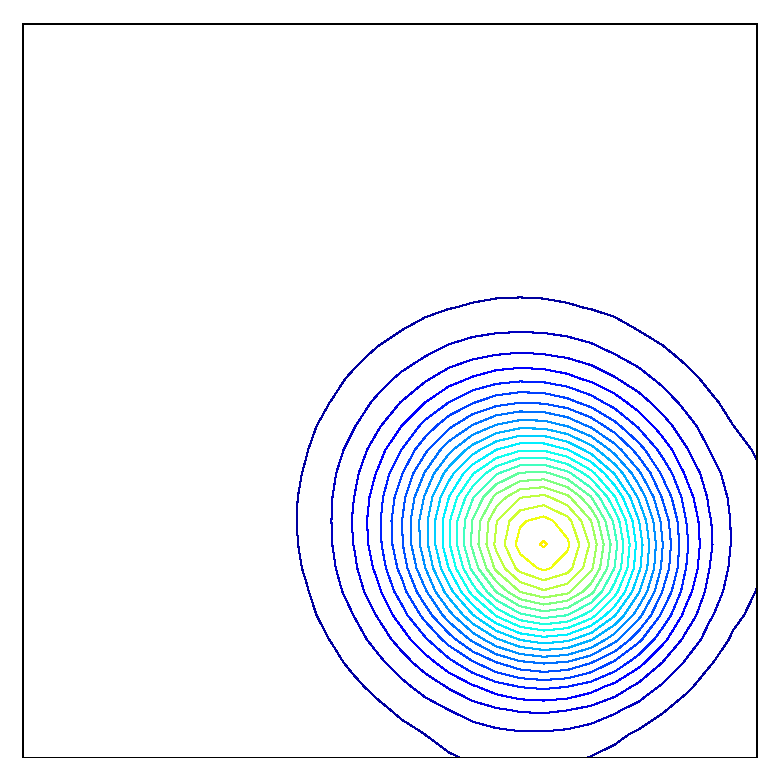
\includegraphics[width=1.6cm]{images/bump_beta/bump_beta_75_iso_29}&
\hspace{-0.45cm}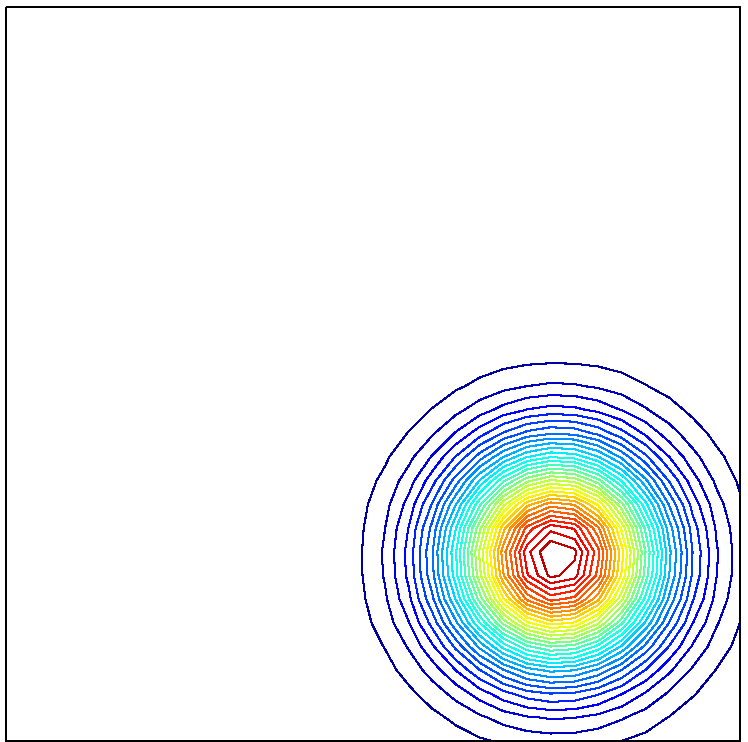
\includegraphics[width=1.6cm]{images/bump_beta/bump_beta_75_iso_33}\\
\sidecap{$\beta=1$ } &\hspace{-0.45cm}
%\animategraphics[palindrome=true,width=1.6cm]{6}{images/bump_anim/bump_beta1_iso_}{01}{33}&
%\movie[mouse=true,palindrome=true]{\includegraphics[width=1.6cm]{images/bump_beta/bump_beta1_iso_01}}{images/bump_beta/beta_1.avi}&
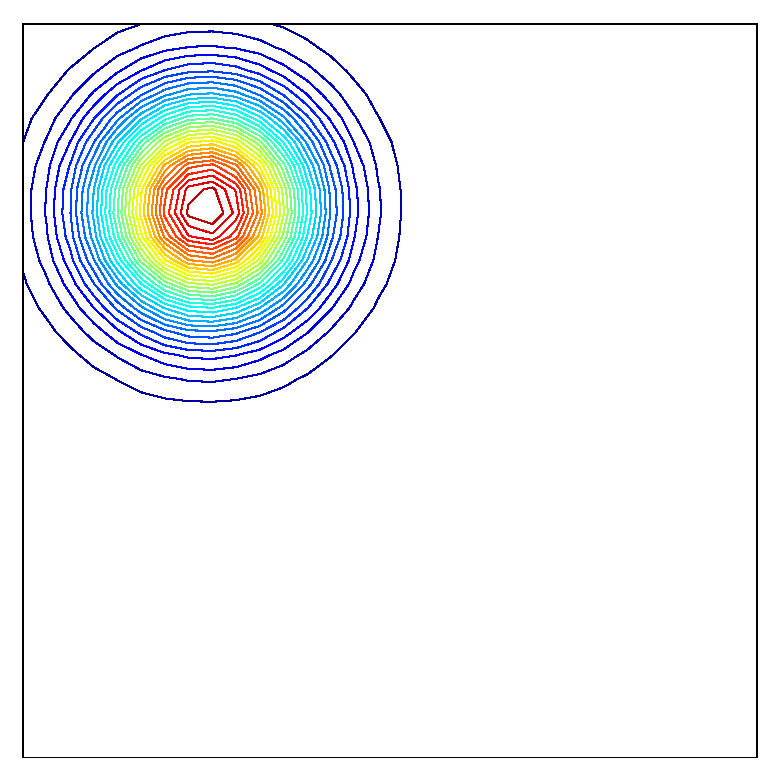
\includegraphics[width=1.6cm]{images/bump_beta/bump_beta_100_iso_01}&
\hspace{-0.45cm}\includegraphics[width=1.6cm]{images/bump_beta/bump_beta_100_iso_05}&
\hspace{-0.45cm}\includegraphics[width=1.6cm]{images/bump_beta/bump_beta_100_iso_09}&
\hspace{-0.45cm}\includegraphics[width=1.6cm]{images/bump_beta/bump_beta_100_iso_13}&
\hspace{-0.45cm}\includegraphics[width=1.6cm]{images/bump_beta/bump_beta_100_iso_17}&
\hspace{-0.45cm}\includegraphics[width=1.6cm]{images/bump_beta/bump_beta_100_iso_21}&
\hspace{-0.45cm}\includegraphics[width=1.6cm]{images/bump_beta/bump_beta_100_iso_25}&
\hspace{-0.45cm}\includegraphics[width=1.6cm]{images/bump_beta/bump_beta_100_iso_29}&
\hspace{-0.45cm}\includegraphics[width=1.6cm]{images/bump_beta/bump_beta_100_iso_33}\\
&\hspace{-0.45cm}$t=0$&\hspace{-0.45cm}$t=1/8$&
\hspace{-0.45cm}$t=1/4$&\hspace{-0.45cm}$t=3/8$&
\hspace{-0.45cm}$t=1/2$&\hspace{-0.45cm}$t=5/8$&
\hspace{-0.45cm}$t=3/4$&\hspace{-0.45cm}$t=7/8$&\hspace{-0.45cm}$t=1$\vspace{-0.2cm}
\end{tabular}
%\includegraphics[trim=100 10 100 10,clip,width=\textwidth]{./images/convergence_bump}
\caption{\label{fig:generalized_bump} 
Display of the level sets of $\iter{f}(\cdot,t)$ for several value of $t$ and $\be$ (note that for $t=0$ and $t=1$, this corresponds to $f^0$ and $f^1$).}
\end{center}
\end{figure}

Figure~\ref{fig:evol_bump_beta} shows for $\beta = 1/2$ and $\be = 3/4$ the evolution of the cost function with the iterations index $\ell$, together with the convergence of the estimate to the reference solution $(m^\star,f^\star)$ (obtained after $10^5$ iterations of the PD algorithm). We can observe that the behavior of the process with $\beta \in ]0,1[$ is different than the one observed for $\beta=1$ in Figure \ref{fig:comp_bump}. Indeed, we observe a faster convergence of the algorithms, which is consistent with the fact that $\Jfunc_\bet$ becomes more and more strongly convex as $\be$ approaches $1/2$ (see \eqref{hessian}). 

\renewcommand{\sidecap}[1]{ {\begin{sideways}\parbox{4cm}{\centering #1}\end{sideways}} }

\begin{figure}[!ht]
\begin{center}
\begin{tabular}{lccc}
\sidecap{$\beta=0.5$ } &
\hspace{-0.3cm}\includegraphics[trim=30 10 40 20,clip,width=0.31\textwidth]{images/J_beta05}&
\hspace{-0.5cm}\includegraphics[trim=30 10 40 20,clip,width=0.31\textwidth]{images/Evol_m_beta_05}&
\hspace{-0.5cm}\includegraphics[trim=30 10 40 20,clip,width=0.31\textwidth]{images/Evol_f_beta_05}\\
\sidecap{$\beta=3/4$ } &
\hspace{-0.3cm}\includegraphics[trim=30 10 40 20,clip,width=0.31\textwidth]{images/J_beta075}&
\hspace{-0.5cm}\includegraphics[trim=30 10 40 20,clip,width=0.31\textwidth]{images/Evol_m_beta_075}&
\hspace{-0.5cm}
\includegraphics[trim=30 10 40 20,clip,width=0.31\textwidth]{images/Evol_f_beta_075}\vspace{0.1cm}\\
&\hspace{-0.3cm}$\Jfunc_\bet( \iter{m},\iter{f} )$&\hspace{-0.5cm}$\norm{m^\star-\iter{m}}$&\hspace{-0.5cm}$\norm{f^\star-\iter{f}}$ \vspace{-0.2cm}
\end{tabular}
\caption{\label{fig:evol_bump_beta} At each iteration $\ell$, we plot the value of the cost function $\Jfunc_\bet(\iter{m},\iter{f})$ and the distance between the reference solution $(m^\star,f^\star)$ and the estimation $(\iter{m},\iter{f})$. The first (resp. second) row presents the result with $\beta=1/2$ (resp. $\bet=3/4$).}
\end{center}
\end{figure}

As a second example, we show in Figure~\ref{fig:generalized_MK} the different morphings obtained between pictures of Gaspard Monge and Leonid Kantorovich. The grayscale representation scales linearly between black (value of 0) and white (value of 1)  and the dimensions are $N+1=75$, $M+1=100$, $P+1=60$, $M$ being the number of discrete points in the second spatial dimension.

\renewcommand{\sidecap}[1]{ {\begin{sideways}\parbox{1.9cm}{\centering #1}\end{sideways}} }
\begin{figure}[!ht]
\begin{center}
\begin{tabular}{cccccccc}
\sidecap{$\beta=0$ } &\hspace{-0.45cm}
%\animategraphics[palindrome=true,width=1.9cm]{102}{images/MK/MK_beta0_}{01}{61}&
%\movie[mouse=true,palindrome=true]{\includegraphics[width=1.9cm]{images/MK/MK_beta0_01}}
%\includegraphics[width=1.9cm]
%{images/MK/MK_000.avi}&
\includegraphics[width=1.9cm]{images/MK/MK_beta0_01}&
\hspace{-0.35cm}\includegraphics[width=1.9cm]{images/MK/MK_beta0_11}&
\hspace{-0.35cm}\includegraphics[width=1.9cm]{images/MK/MK_beta0_21}&
\hspace{-0.35cm}\includegraphics[width=1.9cm]{images/MK/MK_beta0_31}&
\hspace{-0.35cm}\includegraphics[width=1.9cm]{images/MK/MK_beta0_41}&
\hspace{-0.35cm}\includegraphics[width=1.9cm]{images/MK/MK_beta0_51}&
\hspace{-0.35cm}\includegraphics[width=1.9cm]{images/MK/MK_beta0_61}\\
\sidecap{$\beta=0.25$ } &\hspace{-0.45cm}
%\animategraphics[palindrome=true,width=1.9cm]{12}{images/MK/MK_beta25_}{01}{61}&
%\movie[mouse=true,palindrome=true]{\includegraphics[width=1.9cm]{images/MK/MK_beta25_01}}
%\includegraphics[width=1.9cm]
%{images/MK/MK_25.avi}&
\includegraphics[width=1.9cm]{images/MK/MK_beta025_01}&
\hspace{-0.35cm}\includegraphics[width=1.9cm]{images/MK/MK_beta025_11}&
\hspace{-0.35cm}\includegraphics[width=1.9cm]{images/MK/MK_beta025_21}&
\hspace{-0.35cm}\includegraphics[width=1.9cm]{images/MK/MK_beta025_31}&
\hspace{-0.35cm}\includegraphics[width=1.9cm]{images/MK/MK_beta025_41}&
\hspace{-0.35cm}\includegraphics[width=1.9cm]{images/MK/MK_beta025_51}&
\hspace{-0.35cm}\includegraphics[width=1.9cm]{images/MK/MK_beta025_61}\\
\sidecap{$\beta=0.5$ } &\hspace{-0.45cm}
%\animategraphics[palindrome=true,width=1.9cm]{12}{images/MK/MK_beta05_}{01}{61}&
%\movie[mouse=true,palindrome=true]{\includegraphics[width=1.9cm]{images/MK/MK_beta05_01}}
%\includegraphics[width=1.9cm]
%{images/MK/MK_50.avi}&
\includegraphics[width=1.9cm]{images/MK/MK_beta05_01}&
\hspace{-0.35cm}\includegraphics[width=1.9cm]{images/MK/MK_beta05_11}&
\hspace{-0.35cm}\includegraphics[width=1.9cm]{images/MK/MK_beta05_21}&
\hspace{-0.35cm}\includegraphics[width=1.9cm]{images/MK/MK_beta05_31}&
\hspace{-0.35cm}\includegraphics[width=1.9cm]{images/MK/MK_beta05_41}&
\hspace{-0.35cm}\includegraphics[width=1.9cm]{images/MK/MK_beta05_51}&
\hspace{-0.35cm}\includegraphics[width=1.9cm]{images/MK/MK_beta05_61}\\
\sidecap{$\beta=3/4$ } &\hspace{-0.45cm}
%\animategraphics[palindrome=true,width=1.9cm]{12}{images/MK/MK_beta75_}{01}{61}&
%\movie[mouse=true,palindrome=true]{\includegraphics[width=1.9cm]{images/MK/MK_beta75_01}}
%\includegraphics[width=1.9cm]
%{images/MK/MK_75.avi}&
\includegraphics[width=1.9cm]{images/MK/MK_beta075_01}&
\hspace{-0.35cm}\includegraphics[width=1.9cm]{images/MK/MK_beta075_11}&
\hspace{-0.35cm}\includegraphics[width=1.9cm]{images/MK/MK_beta075_21}&
\hspace{-0.35cm}\includegraphics[width=1.9cm]{images/MK/MK_beta075_31}&
\hspace{-0.35cm}\includegraphics[width=1.9cm]{images/MK/MK_beta075_41}&
\hspace{-0.35cm}\includegraphics[width=1.9cm]{images/MK/MK_beta075_51}&
\hspace{-0.35cm}\includegraphics[width=1.9cm]{images/MK/MK_beta075_61}\\
\sidecap{$\beta=1$ } &\hspace{-0.45cm}
%\animategraphics[palindrome=true,width=1.9cm]{12}{images/MK/MK_beta1_}{01}{61}&
%\movie[mouse=true,palindrome=true]{\includegraphics[width=1.9cm]{images/MK/MK_beta1_01}}
%\includegraphics[width=1.9cm]
%{images/MK/MK_100.avi}&
\includegraphics[width=1.9cm]{images/MK/MK_beta1_01}&
\hspace{-0.35cm}\includegraphics[width=1.9cm]{images/MK/MK_beta1_11}&
\hspace{-0.35cm}\includegraphics[width=1.9cm]{images/MK/MK_beta1_21}&
\hspace{-0.35cm}\includegraphics[width=1.9cm]{images/MK/MK_beta1_31}&
\hspace{-0.35cm}\includegraphics[width=1.9cm]{images/MK/MK_beta1_41}&
\hspace{-0.35cm}\includegraphics[width=1.9cm]{images/MK/MK_beta1_51}&
\hspace{-0.35cm}\includegraphics[width=1.9cm]{images/MK/MK_beta1_61}\\
&\hspace{-0.45cm}$t=0$&\hspace{-0.45cm}$t=1/6$&
\hspace{-0.45cm}$t=1/3$&\hspace{-0.45cm}$t=1/2$&
\hspace{-0.45cm}$t=2/3$&\hspace{-0.45cm}$t=5/6$&
\hspace{-0.45cm}$t=1$\vspace{-0.1cm}
\end{tabular}
%\includegraphics[trim=100 10 100 10,clip,width=\textwidth]{./images/convergence_bump}
\caption{\label{fig:generalized_MK} 
Evolution of $\iter{f}(\cdot,t)$ for several value of $t$ and $\be$.
 The first and last columns represent the data $f^0$ and $f^1$. The intermediate ones present the reference solution $f^*(t)$ for successive times $t=i/6$, $i=1\cdots 5$. 
 Each line illustrates $f^*$ for different values $\beta=j/4$, $j=0\cdots 4$ of the generalized cost function. }
%{\it Please click on the first image of each line to visualize the continuous morphings}.}
\end{center}
\end{figure}


%%%%%%%%%%%%%%%%%%%%%%%%%%%%%%%%%%%%%%%%%%%%%%%%%%%%%%%%%%%%%%%%
%%%%%%%%%%%%%%%%%%%%%%%%%%%%%%%%%%%%%%%%%%%%%%%%%%%%%%%%%%%%%%%%
%%%%%%%%%%%%%%%%%%%%%%%%%%%%%%%%%%%%%%%%%%%%%%%%%%%%%%%%%%%%%%%%
\subsection{Riemannian Transportation}
\label{subsec-riemanian-examples}

We investigate in this section the approximation of a displacement interpolation for a ground cost being the squared geodesic distance on a Riemannian manifold. This is achieved by solving~\eqref{eq-optim-bb-gen} with $\be=1$ but a non-constant weight map $w$.


We exemplify this setting by considering optimal transport with obstacles, which corresponds to choosing weights $w$ that are infinity on the obstacle $\Oo \subset \RR^d \times \RR$, i.e. 
\eq{
	\foralls k \in \Gc, \quad w_k = 1 + \iota_{\Cc}(x_k,t_k) \in \{1,+\infty\}.
}
Note that the obstacles can be dynamic, i.e. the weight $w$ needs not to be constant in time. 

Figure~\ref{labyrinthe} shows a first example where $\Oo$ is a 2-D ($d=2$) static labyrinth map (the walls of the labyrinth being the obstacles, and are displayed in black). We use a $50 \times 50 \times 100$ discretization grid of the space-time domain $[0,1]^3$ and the input measures $(f^0,f^1)$ are Gaussians  with standard deviations equal to $0.04$. For Gaussians with such a small variance, this example shows that the displacement interpolation is located  closely to the geodesic path between the centers of the gaussians.


\begin{figure}[!ht]
\begin{center}
\begin{tabular}{ccccc}
%\animategraphics[palindrome=true,width=3.2cm]{12}{obstacle_mobile/bump_obstacle5_iso_0}{01}{65}&
\hspace{-0.2cm}\includegraphics[width=3cm]{images/labyrinthe/bump_obstacle5_iso_001}&
\hspace{-0.4cm}\includegraphics[width=3cm]{images/labyrinthe/bump_obstacle5_iso_012}&
\hspace{-0.4cm}\includegraphics[width=3cm]{images/labyrinthe/bump_obstacle5_iso_023}&
\hspace{-0.4cm}\includegraphics[width=3cm]{images/labyrinthe/bump_obstacle5_iso_034}&
\hspace{-0.4cm}\includegraphics[width=3cm]{images/labyrinthe/bump_obstacle5_iso_045}\\
\hspace{-0.2cm}$t=0$&
\hspace{-0.4cm}$t=1/9$&
\hspace{-0.4cm}$t=2/9$&
\hspace{-0.4cm}$t=1/3$&
\hspace{-0.4cm}$t=4/9$\\
\hspace{-0.2cm}\includegraphics[width=3cm]{images/labyrinthe/bump_obstacle5_iso_056}&
\hspace{-0.4cm}\includegraphics[width=3cm]{images/labyrinthe/bump_obstacle5_iso_067}&
\hspace{-0.4cm}\includegraphics[width=3cm]{images/labyrinthe/bump_obstacle5_iso_078}&
\hspace{-0.4cm}\includegraphics[width=3cm]{images/labyrinthe/bump_obstacle5_iso_089}&
\hspace{-0.4cm}\includegraphics[width=3cm]{images/labyrinthe/bump_obstacle5_iso_101}\\
\hspace{-0.2cm}$t=5/9$&
\hspace{-0.4cm}$t=2/3$&
\hspace{-0.4cm}$t=7/9$&
\hspace{-0.4cm}$t=8/9$&\hspace{-0.35cm}$t=1$
\end{tabular}
\caption{\label{labyrinthe} 
Evolution of $\iter{f}(\cdot,t)$ for several values of $t$, using a Riemannian manifold with weights $w_k$ (constant in time) restricting the densities to lie within a 2-D static labyrinth map.  }
\end{center}
\end{figure}


Figure~\ref{labyrinthe2} shows a more complicated setting that includes a labyrinth with moving walls: a wall appears at time $t=1/4$ and another one disappears at time $1/2$. The difference with respect to the previous example is the fact that $w$ is now time dependent. This simple modification has a strong impact on the displacement interpolation. Indeed, the speed of propagation of the mean of the density is not constant anymore since the density measure is confined in a small area surrounded by walls for $t \in [1/4,1/2]$.


\begin{figure}[!ht]
\begin{center}
\begin{tabular}{ccccc}
%\animategraphics[palindrome=true,width=3.2cm]{12}{labyrinthe4/bump_obstacle5_iso_}{001}{101}&
\hspace{-0.2cm}\includegraphics[width=3cm]{images/labyrinthe4/bump_obstacle5_iso_001}&
\hspace{-0.4cm}\includegraphics[width=3cm]{images/labyrinthe4/bump_obstacle5_iso_012}&
\hspace{-0.4cm}\includegraphics[width=3cm]{images/labyrinthe4/bump_obstacle5_iso_023}&
\hspace{-0.4cm}\includegraphics[width=3cm]{images/labyrinthe4/bump_obstacle5_iso_034}&
\hspace{-0.4cm}\includegraphics[width=3cm]{images/labyrinthe4/bump_obstacle5_iso_045}\\
\hspace{-0.2cm}$t=0$&
\hspace{-0.4cm}$t=1/9$&
\hspace{-0.4cm}$t=2/9$&
\hspace{-0.4cm}$t=1/3$&
\hspace{-0.4cm}$t=4/9$\\
\hspace{-0.2cm}\includegraphics[width=3cm]{images/labyrinthe4/bump_obstacle5_iso_056}&
\hspace{-0.4cm}\includegraphics[width=3cm]{images/labyrinthe4/bump_obstacle5_iso_067}&
\hspace{-0.4cm}\includegraphics[width=3cm]{images/labyrinthe4/bump_obstacle5_iso_078}&
\hspace{-0.4cm}\includegraphics[width=3cm]{images/labyrinthe4/bump_obstacle5_iso_089}&
\hspace{-0.4cm}\includegraphics[width=3cm]{images/labyrinthe4/bump_obstacle5_iso_101}\\
\hspace{-0.2cm}$t=5/9$&
\hspace{-0.4cm}$t=2/3$&
\hspace{-0.4cm}$t=7/9$&
\hspace{-0.4cm}$t=8/9$&\hspace{-0.35cm}$t=1$
\end{tabular}
\caption{\label{labyrinthe2} Evolution of $\iter{f}(\cdot,t)$ for several values of $t$, using a Riemannian  manifold with weights $w_k$ (evolving in time) restricting the densities to lie within a 2-D dynamic labyrinth map (i.e. with moving walls). }
\end{center}
\end{figure}
